\documentclass{./cls/spbau-diploma}

% Для удобной раздельной компиляции: скомпилированы будут только те главы, которые перечислены
% в аргументе \includeonly
% \includeonly{annotation}

\begin{document}

\filltitle{ru}{
    chair              = {Кафедра математических и информационных технологий},
    title              = {TODO},
    % Здесь указывается тип работы. Возможные значения:
    %   coursework - Курсовая работа
    %   diploma - Диплом специалиста
    %   master - Диплом магистра
    %   bachelor - Диплом бакалавра
    type               = {master},
    position           = {студента},
    group              = TODO,
    author             = {TODO},
    supervisorPosition = {TODO},
    supervisor         = {TODO},
    reviewerPosition   = {TODO},
    reviewer           = {TODO},
    chairHeadPosition  = {д.\,ф.-м.\,н., профессор},
    chairHead          = {Омельченко А.\,В.},
    % university = {САНКТ-ПЕТЕРБУРГСКИЙ АКАДЕМИЧЕСКИЙ УНИВЕРСИТЕТ},
    % faculty = {Центр высшего образования},
    % city = {Санкт-Петербург},
    % year             = {2013}
}


\maketitle
\tableofcontents

\section*{Аннотация}

Это аннотация. Тут будет много умных вещей.
\section*{Введение}

Актуальность задачи статического анализа кода, на сегодняшний день, уже не вызывает ни у кого сомнения. Статический анализ обнаруживает ошибки в коде (как связанные с логикой, так и связанные с быстродействием, стилем), поставляет информацию, необходимую для проведения оптимизаций в коде, его рефакторинге. Статические анализаторы используются как в узкоспециализированных инструментах, основной задачей которых является непосредственный анализ кода, так и в качестве составной части других, более крупных систем -- таких как компиляторы, IDE, оптимизаторы.

Одним из возможных методов статического анализа являются \term{системы эффектов}. Эффект -- это некоторое воздействие вычисления (функции, метода, подпрограммы) на состояние вычислителя. Простым примером эффекта является запись или чтение в разделяемую подпрограммами переменную, или же тот факт, что функция может бросить некоторое исключение (последний тип эффектов был реализован в языке \lang{Java} в виде механизма проверяемых исключений). Система эффектов отвечает за корректный учёт всех эффектов, их взаимодействие друг с другом, а также другие действия с ними (вывод, проверка, и т.д.)

Важным свойством, которому будет уделено значительно внимание, является то, что при анализе кода эффекты часто \textit{наблюдаются}. Так, в блоке \code{catch} в \lang{Java} мы наблюдаем тот эффект, что некоторая функция сгенерировала исключение. Однако в классических системах эффектов, это наблюдение не дает анализатору никакой информации. Вместе с тем, если бы было известно, какие условия вызывают такой эффект, то из факта наблюдения можно было бы сделать вывод, что окружение удовлетворяет поставленным условиям, тем самым извлекая больше информации из кода. 

В связи с этом, мы предлагаем систему эффектов, расширенную добавлением условных эффектов, про которые известны вызывающие их условия. Это позволяет описать в рамках системы более широкий набор функций и соответствующих им эффектов, и, что наиболее важно, извлечь из использования системы значительно больше пользы при тесной интеграции с компиляторами и/или IDE. 

В качестве демонстрации применения предложенной системы, будет изучена польза от рассмотрения условных эффектов на примере языка \lang{Kotlin}. Данный язык интересен из-за механизма <<умных приведений типов>> (англ. \eng{smartcasts}) -- если в некотором участке кода статически гарантированно, что переменная имеет более частный тип, то компилятор сделает приведение к этому типу автоматически. Этот механизм естественным образом дополняет систему условных эффектов: пронаблюдав эффект и узнав некоторую типовую информацию о переменных в окружении, можно сделать умное приведение типов там, где раньше оно не делалось или же было вовсе невозможно. 

Таким образом, в работе будет рассмотрен ряд эффектов, естественным образом возникающих из предметной области -- в частности, эффекты, сообщающие о типе или значении переменных окружения. Кроме того, в работе будет показано, как ввести эффекты, сообщающие о том, что некоторая процедура была вызвана детерминированное количество раз. Данные эффекты могут быть очень полезны в комбинации с другими видами анализа, нуждающимися в подобных гарантиях для сохранения консервативности (например, анализ инициализации переменных).

Также будут рассмотрены вопросы комбинации условных эффектов при вложенных вызовах. Отдельное внимание будет уделено проблеме работы с эффектами в присутствии частичных вычислений.

В заключение, будет произведен анализ применимости систем условных эффектов, будут намечены направления развития данного исследования.


\section{Глава 1}

\subsection{Теоретические основы}

В данной работе нам понадобится ряд формальных определений и терминов, которые мы будем использовать в дальнейшем. 

\subsubsection{Понятие подпрограммы}

Первым делом, условимся использовать термины \term{подпрограмма}, \term{функция}, \term{метод}, \term{процедура} взаимозаменяемо, в смысле, интуитивно соответствующему англ. \eng{callable}. Более формально:

\begin{definition}
    \term{Подпрограммой} (функцией, методом, процедурой) будем называть выделенную последовательность инструкций, в которую может быть передано управление, и которая по завершению возвращает его в место вызова \cite{Wheeler52}.
\end{definition}

Отметим, что также в это определение укладываются все объекты, на которых можно произвести непосредственный вызов, если таковые поддерживаются языком -- например, объекты, с переопределенным методом \code{invoke} в \lang{Kotlin}, \code{apply} в \lang{Scala}, \code{\_\_call\_\_} в \lang{Python} и т.д.






\newpage



\subsection{Обзор существующих решений}


\subsubsection{Системы эффектов}

Системы эффектов появились в конце 80-ых годов как логичное развитие систем типов. Из-за этого, между системами типов и системами эффектов существует естественная связь, служащая источником для различных интуиций и полезных параллелей. Поскольку осознание этой связи значительно облегчает понимание любых фактов и свойств систем эффектов, ниже будет вкратце описано, откуда эта связь появляется.

\bigskip

В компьютерных программах существует два основополагающих понятия: это объекты, которые хранят информацию, и функции, которые что-то делают с объектами

Системы типов отвечают за информацию об объектах. Мы можем написать нечто вроде \code{a: Int}, и это будет означать, что между программистом и компилятором установлено некоторое соглашение относительно того, какого рода информация соответствует этой переменной -- в зависимости от конкретного языка, это может означать, например, что в \code{a} хранится 32-битное знаковое целое число. Более конкретные спецификации могут даже устанавливать соглашение о том, как именно кодируется это число и как оно хранится в памяти.

Но мощь систем типов ограничена, когда речь заходит о функциях -- что и неудивительно, т.к. тип говорит о свойствах объекта, а не процедур. Отчасти проблема решается сигнатурами, но по сути, это всего лишь информация об аргументах и возвращаемом объекте, но никак не о том, что с ними делает функция. Так, сигнатура \code{void doSomething()} в \lang{Java} не дает никакой информации, и программисту остается лишь надеяться на адекватное название и комментарии в коде.

Отсюда и рождается идея эффектов и систем эффектов. Эффект для процедуры -- это тоже самое, что тип для объекта. Так, в одной из первых работ по системам эффектов, дается следующее определение:

\begin{definition}
	\term{Эффектом} выражения называется краткое описание всех наблюдаемых побочных эффектов, которые это выражение может вызвать при вычислении \cite{Luc88}.
	\label{def-effect}
\end{definition}

Традиционно для подобных исследований, авторы немного лукавят и не определяют <<побочный эффект>> строго, надеясь на интуицию читателя (в их оправдание скажем, что интуиция, скорее всего, не подведет). В главе 2 мы четко разберемся со всеми этими понятиями и дадим точные определения. Пока же можно считать, что <<побочный эффект>> соответствует некоторому изменению в памяти программы.


Тесная связь между системами типов и системами эффектов сходу дает значительное количество полезных наблюдений. Чтобы подчеркнуть двойственность между этими двумя системами, эти наблюдения оформлены в таблицу \ref{types-effects-comparison}

\begin{table}
\begin{tabular}{ | p{0.4\linewidth} | p{0.4\linewidth} | }
	\hline
	Системы типов & Системы эффектов \\\hline

	Помогают предотвращать ошибки -- например, от сохранения строкового значения в тип \code{Int}.
	&
	Помогают предотвращать ошибки -- например, от использования функции, которая бросает исключение, вне блока \code{try-catch}.
	\\\hline

	Помогают компилятору -- например, знание о типе переменной может позволить хранить ее в памяти более оптимально.
	&
	Помогают компилятору -- например, знание о том, в какие переменные пишет функция и какие читает, может позволить переупорядочивание кода, ранее невозможное.
	\\\hline


	\multicolumn{2}{| p{0.8\linewidth + 2\tabcolsep}|}{Типы/эффекты могут быть либо явно написаны пользователем, либо выведены автоматически}

    \\\hline

    \multicolumn{2}{| p{0.8\linewidth + 2\tabcolsep} |}{Бывает полезной возможность введения пользовательских типов/эффектов}
	\\\hline

\end{tabular}
\label{types-effects-comparison}
\caption{Сравнение типов и эффектов}
\end{table}

\bigskip

Основопологающей работой является уже упомянутая несколько раз статья Lucassen, Gifford <<Polymorphic effect system>> (1988) \cite{Luc88}. В ней авторы описывают основы систем эффектов, предлагают формализм, схожий с формализмом систем типов, позволяющий описывать эффекты. Данное исследование является в большей степени математической формализацией концепта эффектов, нежели руководством к тому, как использовать этот концепт на практике.

С точки зрения практики, очень интересной является статья Greenhouse, Boyland <<An Object-Oriented Effect System>> (1999) \cite{Green99}. В ней авторы задаются уже вполне жизненными и насущными вопросами о применении систем эффектов в условиях объекто-ориентированного \lang{Java}-подобного языка. Так, рассмотрены проблемы наследования эффектов, инкапсуляции в присутствии эффектов.

Cледует отметить, что в этих двух статьях, как и в большинстве других, авторы уделают крайне мало внимания расширяемости системы по типам эффектов, и как следствие, по типам анализа, рассматривая простые \code{read/write} эффекты чтения-записи в перменную, которые отличаются очень простыми правилами комбинирования. 

В качестве редкого примера эффектов, более интересных с концептуальной точки зрения, можно привести многопоточные условные эффекты из работы Flanagan, Freund, Lifshin <<Types for atomicity: Static Checking and Inference for Java>> (2008) \cite{Flanagan08}. Авторы ставят цель разработать систему эффектов, способную обнаруживать ошибки в программах на \lang{Java}, связанные с многопоточностью. В связи с этим вводится класс эффектов, связанных с различными типами многопоточного взаимодействия. Также очень интересно отметить, что здесь появляются некоторые простые условные эффекты, связанные с тем, что поведение многопоточных методов почти всегда зависит от владения той или иной блокировкой. Авторы сталкиваются с некоторыми проблемами, свойственными условным эффектам -- в частности, экспоненциальный взрыв длины аннотаций при последовательном комбинировании эффектов (мы подробней будем говорить об этом в главе 2). 

Следует отметить замечательную особенность эффектов -- вычислительная сложность анализа зависит от количества аннотаций эффектов и их типов, но не от длины кода (разумеется, в отсутствии автоматического вывода эффектов). Таким образом, пользователь подобной системы <<платит только за то, что использует>>: работа с проектом без аннотаций будет очень похожа на то, как если бы системы эффектов не было вовсе. Более того, пользователь может захотеть проаннотировать только некоторую подсистему, либо же использовать ровно один простой тип эффектов (какие-нибудь проверяемые исключения) -- в том и в другом случае, он может легко получить желаемый результат без значительной платы процессорным временем. 


\bigskip

Взглянем теперь в сторону практических реализаций систем эффектов.

Реализацией идеи систем эффектов по оригинальной статье является язык программирования FX-87 \cite{FX87}. К несчастью, этот язык на сегодняшний день уже не поддерживается и развивается (чему он, вероятно, в значительной степени обязан в высшей степени нечитаемому синтаксису). Кроме того, данный язык является функциональным, что еще более уменьшает актуальность этой реализации для настоящего исследования.

Намного более практико-ориентированной, и потому более интересной, явлется \name{Checker Framework} \cite{checker-framework}. Это фреймворк, построенный на основе JSR-308 \cite{JSR308}, и позволяющий организовывать небольшие системы эффектов на основе \lang{Java}-аннотаций. Кроме того, возможно аннотирование объектов. Фреймворк предоставляет набор готовых аннотаций, равно как и возможность задавать собственные.

\name{Checker Framework} построен на понятии \name{checker}-ов -- небольших модулей, отвечающих за решение одной конкретной задачи анализа (с чисто технической точки зрения, каждый такой модуль является процессором аннотаций). \name{Checker}-ы независимы друг от друга, и могут добавляться в систему по мере необходимости, что обеспечивает масштабируемость по типам анализа.

Полезным наблюдением, которое можно извлечь из принципа устройства \name{Checker Framework} является тот факт, что подавляющее большинство эффектов нетривиально взаимодействуют только с эффектами такого же типа и никак не влияют на все остальные - именно на этом основывается модульная структура с \name{checker}-ами. Это дает очень важное понимание того, насколько хорошо ведут себя системы эффектов при масштабировании -- добавление нового эффекта никак не зависит от количества уже существующих эффектов (при условии, что он с ними не взаимодействует, что чаще всего действительно так). Это второе очень важное свойство систем эффектов, помимо независимости вычислительной сложности анализа от длины кода.








\subsubsection{Контракты}

Подходом к той же самой проблеме, но несколько с другой стороны являются \term{контракты}.

\begin{definition}
	\label{def-contract}
	\term{Контракт} -- это формальная, точная и проверяемая спецификация программной единицы, описывающая ее взаимодействие с другими программными единицами \cite{Meyer92}
\end{definition}

Чаще всего в качестве программной единицы используется функция. Контракты для функций описываются предусловием, постусловием и инвариантом. Предусловие -- это набор ограничений на окружение, которые функция ожидает видеть выполненными. Постусловие -- это условия, которые функция обязуется выполнить, если было выполнено предусловие. Инвариант -- это условия, которые функция обязуется выполнять всегда.

Внимательно вдумавшись в определение \ref{def-contract}, можно заметить, что оно очень близко по смыслу к определению \ref{def-effect}. Это и не удивительно, т.к. оба метода ставят своей целью явно специфицировать межпроцедурные взаимодействия.  Отличие контрактов от эффектов заключается больше в синтаксисе записи и терминологии, нежели в концептуальных различиях. В достаточно мощной системе эффектов можно выразить понятие контракта, и обратно, с помощью контрактов и некоторого числа дополнительных конструкций можно записать эффекты функции. Разумеется, некоторые эффекты легче укладываются в концепцию контрактов, и наоборот. 

Несмотря на схожесть контрактов и эффектов с точки зрения выразительности, между ними есть разница, если задуматься о чисто практических вопросах -- а именно, о том, какого рода утверждения нужно будет чаще формализовывать в рамках системы анализа. 

Системы эффектов часто являются интуитивно понятными, когда каждый эффект говорит о наличии либо отсутствии некоторого четко определенного и кратко описываемого свойства у функции -- возможности бросить исключение, чистоты, и т.д. Само по себе свойство может быть довольно нетривиальным -- например, если пытаться формализовать понятие чистоты не используя непосредственно термин <<чистая функция>>, то придется формализовать довольно длинную мысль: <<на одним и том же наборе входных аргументов функция всегда возвращает одно и то же значение, и при этом выполнение функции никогда не вызывает наблюдаемых побочных эффектов>>. Однако важно, что будучи однажды введенным, это свойство записывается кратко и емко.

Контракты же удобны, если центральные понятия -- предусловия и постусловия -- будут часто использоваться. То же самое понятие чистоты функции никак не связано с предусловиями и постусловиями, и даже с понятием инварианта -- это просто неотъемлемое свойство функции. Некоторым расширением синтаксиса контрактов, конечно, можно его выразить ровно также, как и в эффектов -- но если в предметной области все утверждения похожи по своему устройству на чистоту, то смысла в контрактах остается не много.

Подводя итог, можно сказать, что в целом по своим свойствам контракты очень похожи на эффекты, а выбор конкретного подхода должен зависеть от предметной области и от того, какого рода утверждения будут чаще использоваться в итоговой системе. 






\subsubsection{Анализ потока данных}

Анализ потока данных (англ. \eng{data-flow analysis}) является методом статического анализа, возникшим в результате развития компиляторов, и, как следствие, потребности в эффективном и практичном способе доказательства \emph{некоторых} свойств программы.

Отличие анализа потока данных от тех же языков спецификации заключается в том, что анализ потока данных не пытается доказать корректность программы в целом, а вместо этого сосредотачивается на некоторых, достаточно простых и полезных свойствах, например, константности переменных, типах и аттрибутах переменных, и т.д. \cite{Sharir78}

Мы будем достаточно подробно обсуждать детали работы анализа потока данных чуть позже, здесь же ограничимся тем, что он анализирует непосредственно исходный код. В этом его основное отличие от систем эффектов и контрактов -- анализ потока данных, с одной стороны, работает прозрачно для пользователя, не требуя от него никаких специальных аннотаций. С другой же стороны, это приводит к некоторых техническим ограничениям. В частности, отсутствие исходного кода делает анализ невозможным, что приводит к некоторым проблемам при использовании в языках с раздельной компиляцией.

Кроме того, как несложно догадаться, вычислительная сложность анализа потока данных растет вместе с размером анализируемого кода \cite{Sagiv96}. В связи с этим, на практике наиболее распространен внутрипроцедурный анализ потока данных, т.к. он значительно проще в реализации, и вместе с тем все равно позволяет получать довольно полезные на практике утверждения \cite{dragon-book}.

В контексте данной работы интерес представляет межпроцедурный анализ потока данных. Одним из наиболее логичных и распространенных методов борьбы с возрастающей сложностью при межпроцедурном анализе является <<сжатие>> информации о подпрограммах \cite{Weihl80, Barth78}. Суть достаточно проста -- вместо того, чтобы пытаться <<в лоб>> проанализировать код всей программы, мы заменяем все подпрограммы на некоторые краткие описания ее эффектов и взаимодействий, релевантных для конкретного типа анализа. После этого, межпроцедурный анализ начинает напоминать внутрипроцедурный -- при анализе конкретной подпрограммы, вместо кода использованных в ней других подпрограмм, используются полученные ранее краткие описания.

Как и следует ожидать, итоговые характеристики подобного подхода очень сильно зависят от того, как получаются эти <<краткие описания>>. По этой причине мы не будем подробно анализировать возможные виды межпроцедурного анализа, основанные на этой идее, поскольку этот анализ будет довольно точно следовать анализу конкретного метода, использованного для извлечения кратких описаний.




\subsubsection{Языки спецификаций}

\begin{definition}
	\term{Языком спецификаций} называется формальный язык, призванный описывать свойства и поведение систем на более высоком уровне абстракции, нежели языки программирования.
\end{definition}

Как следует из определения, целью языков спецификации является как можно более подробное формальное описание систем. В связи с этим, большинство современных известных языков спецификации являются очень мощными системами, построенных вокруг фундаментальных понятий алгебры, математической логики, теории типов, теории категорий.

Например, язык спецификаций \name{Z-нотация} (англ. \eng{Z-notation}) основывается на теории множеств, лямбда-исчислении и логики предикатов первого порядка \cite{Z-notation}. Язык \name{CASL} поддерживает логику первого порядка, индукцию, частичные функции, наследование, и др. \cite{CASL}.

Благодаря мощному инструментарию, языки спецификации могут формализовывать довольно сложные и нетривиальные утверждения, связи и взаимодействия в системе. Следует ожидать, что в языках спецификации можно выразить и системы эффектов, и контракты, и это действительно так -- язык \name{Larch} использует ключевые слова \code{require}, \code{ensure} для описания предусловий и постусловий \cite{Larch}

В силу врожденной гибкости и выразительности, языки спецификаций обладают впечатляющей расширяемостью по типам анализа. Ценой же этому становится сложность. Подобные языки вводят значительное количество новых концепций и понятий, а также требуют от пользователя знания фундаментальных теорий, положенных в основу языка (чаще всего, алгебры и математической логики). Спецификации к программам могут быть длиннее и сложнее самих программ. В связи с этим, языки спецификаций в основном находят свое применение в тех областях разработки ПО, где недопустимы даже малейшие сбои и ошибки -- например, при разработке аппаратов радиотерапии \cite{Jacky97}.

Таким образом, языки спецификаций -- это отдельный, готовый инструмент, предназначенный в большей степени для формального доказательства корректности программ, нежели чем для улучшения качества статического анализа. Тем не менее, их выразительность, гибкость, а также в целом возможность воспользоваться готовым решением вроде CASL или Larch может иногда выглядеть довольно заманчиво. 



\newpage



\subsection{Предметная область}

До этого момента мы, в основном, говорили несколько абстрактно и неконкретно. Это и неудивительно, т.к. такие понятия, как <<язык формальной спецификации>> или <<контракты>> являются очень широкими, способными гибко подстраиваться под любую предметную область и ее требования.

Вместе с тем, продолжать дальнейший разговор без предъявления некоторых реальных проблем видится видится крайне малоосмысленным. Поэтому в данном разделе будет рассказана краткая вводная в язык \code{Kotlin} и несколько реальных проблем синтаксического анализа в нем, связанных с межпроцедурным анализом. Это позволит сформулировать несколько несложных требований к разрабатываемой системе, которые будут служить нам базовой проверкой ее адекватности реальным задачам.


\subsubsection{Механизм умных приведений типов}

Важным механизмом, понимание которого необходимо для дальнейшего разговоре о \lang{Kotlin}, является механизм \term{умных приведений типов} (англ. \eng{smartcasts}). 

Очень часто, перед явным приведением типа в коде выполняется проверка на подтип (для того, чтобы такое приведение было безопасным). В \lang{Java} это выглядит примерно следующим образом:

\begin{minted}{java}
if (x instanceof string) {
string s = (string) x;
... usage of s ...
}
\end{minted}

Суть механизма умных приведений типов заключается в том, чтобы облегчить программисту жизнь и выполнить приведение к более частному типу автоматически там, где это безопасно. 

Вот эквивалентный участок кода на \lang{Kotlin}: 

\begin{minted}{kotlin}
if (x is String) {
val len = x.length
}
\end{minted}

Во второй строке произошло автоматические приведение типа, благодаря чему стал возможным доступ к полю \code{String.length}.

Особенно удобно это вместе с \code{when}-конструкцией, которая является более мощным аналогом \code{switch-case} из \code{Java}, в частности, позволяя использовать в \code{Kotlin} синтаксис, напоминающий сравнение с образцом (англ. \code{pattern matching}).

\begin{minted}{kotlin}
when (x) {
is String -> x.length   // x casted to String
is List<Int> -> x.size  // x casted to List
is Double -> x * 2.0    // x casted to Double

}
\end{minted}




\subsubsection{Проблемы механизма умных приведений типов}

Основная проблема заключается в том, что анализ возможности приведения типа выполняется без учета межпроцедурных взаимодействий. Так, давайте вспомним уже знакомую нам функцию проверки на строковый тип:

\begin{minted}{kotlin}
fun isString(x: Any?): Boolean {
return x is String
}
\end{minted}

Теперь если использовать эту функцию в качестве условия условного оператора, то умное приведение типа выполнено не будет:

\begin{minted}{kotlin}
if (isString(x)) {
val s = x as String    // explicit cast needed
}
\end{minted}

Особенно актуальна эта проблема для работы с коллекциями с использованием stream-like API, предоставляемом в \lang{Kotlin}. Так, существует метод \code{filter}, который оставляет в коллекции только те элементы, на которых переданный предикат вернул \code{true}. Этот метод довольно часто используется для того, чтобы оставить в коллекции только объекты определенного типа: \code{list.filter(x -> x is String)} оставит в коллекции \code{list} только строки.

Разумеется, в обоих описанных случаях компилятор не может просто так выполнить умное приведение типа -- для этого ему нужно знать некоторый <<контракт>> вызываемой функции. 

Для \code{isString} нужно знать, что <<\code{isString(x)} возвращает \code{true} тогда и только тогда, когда \code{x} -- \code{String}>>. 

Для \code{filter} нужно знать, что он оставляет в коллекции только те объекты, на которых переданный предикат вернул \code{true}.


\bigskip

Другим распространенным случаем, когда умное приведение типов можно было бы сделать, но оно не делается, являются функции, которые могут завершиться с исключением. 

Рассмотрим следующий пример:

\begin{minted}{kotlin}
assert(x is String)
val s = x as String    // explicit cast needed
\end{minted}

Если мы будем считать, что \code{assert} бросает исключение всегда, когда его условие -- \code{false} (на практике это зависит от ключей окружения, но мы опустим эти детали реализации), тогда во второй строке автоматическое приведение типа может быть безопасно выполнено. Тем не менее, на данный момент компилятор \lang{Kotlin} этого не делает, ровно по тем же причинам, что и в примерах выше -- он не выполняет межпроцедурного анализа, и потому ему не известен контракт <<assert>>. 




\subsubsection{Анализ инициализации переменных}

\lang{Kotlin} поддерживает отложенную инициализацию локальных переменных и будет отслеживать и предупреждать об использовании неинициализированных переменных:

\begin{minted}{kotlin}
val x: Int
// println(x)
x = 5
println(x)
\end{minted}

Если раскомментировать строку 2, то компилятор вполне законно выдаст ошибку об использовании неинициализированной переменной. 

Теперь рассмотрим функцию \code{run}, которая просто вызывает переданную ей лямбду: 
\begin{minted}{kotlin}
fun run(block: () -> Unit): Unit {
block()
}
\end{minted}

Если теперь выполнить отложенную инициализацию переменной внутри лямбды, переданной внутрь \code{run}, то компилятор уже не сможет доказать, что переменная была корректно проинициализированна:

\begin{minted}{kotlin}
val x: Int
run ({ () -> x = 5 })
println(x)
\end{minted}

Компилятор отвергает подобный код, ошибочно сообщая об использовании неинициализированной переменной в строке 3. Причина этого примерно такая же, как и во всех предыдущих примерах: компилятор не знает контракта функции \code{run}, и потому не знает, что лямбда \code{\{ () -> x = 5 \}} будет гарантированно вызвана.

Этот пример умышленно утрирован для простоты объяснения. На самом деле, это вполне актуальная и серьезная проблема, т.к. \code{Kotlin} придерживается философии введения как можно меньшего количества ключевых слов. Это возможно из-за существования лямбд и функций высшего порядка, а также из-за синтаксического сахара, позволяющего передавать лямбду в виде блока, если она передается последней в списке параметров. Именно так реализован аналог ключевого слова \code{synchronized} из \lang{Java}: в \lang{Kotlin} это обычная функция, определенная примерно следующим образом (детали взятия и освобождения блокировки опущены для ясности).

\begin{minted}{kotlin}
fun synchronized(block: () -> Unit): Unit {
... take lock ...
block()
... release lock ...
}
\end{minted}

В пользовательском коде использование этой функции с учетом описанного выше синтаксического сахара выглядит следующим образом:

\begin{minted}{kotlin}
val x: Int
synchornized {
x = 5
}
println(x)
\end{minted}

Точно также, как в примере с \code{run}, компилятор заявляет о том, что в строке 5 переменная \code{x} не инициализирована. Это уже более серьезная проблема, т.к. здесь нельзя обойтись парой избыточных символов, как это было в примере с умными приведениями типа. 
q
Такой случай использования является вполне жизненным и распространенным, и в будущем будет появляться лишь больше функций, похожих на \code{run} и \code{synchronized}. Например, абсолютно также реализована идиома \code{try-with-resources} из \code{Java}, различные функции для работы с корутинами, и т.д.

Для того, чтобы решить это проблему, необходимо некоторым образом донести до компилятора контракт всех таких функций: что они вызывают переданную им лямбду некоторое статически детерминированное число раз. 





\subsection{Актуальность, цель и задачи работы}

Подведем краткий итог проблем, которые мы пронаблюдали в предметной области:

\begin{itemize}
    \item Корнем всех перечисленных выше проблем являются неучтенные межпроцедурные взаимодействия
    
    \item Для того, чтобы корректно дополнить анализ, необходимо извлечь некоторые факты и утверждения о том, как именно работают функции (связь входного и выходного значения, как в \code{isString}, или же информация о поведении функции по отношению к переданным аргументам, как в \code{run})
    
    \item Следует ожидать, что контракты могут становиться весьма нетривиальными, равно как и то, что достаточно простые контракты может оказаться непросто выводить в автоматическом режиме (например, функция может действительно вызывать лямбду ровно один раз, но при этом делать еще множество других нетривиальных вещей, тем самым затрудняя анализ).
\end{itemize}

На основе этих утверждений, можно сформулировать ряд ожидаемых требований:

\begin{enumerate}
	\item Система должна быть способна описывать межпроцедурные взаимодействия с условиями (например, связь между аргументами функции и возвращаемым значением).
	
	\item Система должна поддерживать явные пользовательские аннотации.
	
	\item Система должна быть удобной для интеграции с существующими решениями (компиляторами, IDE).
	
	\item Вычислительная сложность анализа должна позволять работу с крупными проектами (от сотен тысяч строк кода).
	
	\item Система должна по возможности легко расширяться по типам анализа.
\end{enumerate}

Вспомним рассмотренные нами подходы. Их соответствие означенным критериям сведено в таблицу \ref{approaches-analysis}

\begin{table}
\begin{tabular}{ | p{0.15\linewidth} | p{0.15\linewidth} | p{0.15\linewidth} | p{0.15\linewidth} | p{0.20\linewidth} | p{0.15\linewidth} | }
	\hline
					     & Условные контракты & Явные аннотации            & Удобство интеграции & Независимость от длины кода & Расширяемость \\\hline
	
	Анализ потока данных & 	-				  & -						   & +					 & -						   & + 			   \\\hline
	
	Языки спецификаций   & +				  & +						   & -					 & +						   & +			   \\\hline
	
	Эффекты			     & +/- 				  & +						   & +					 & +						   & +   		   \\\hline
	
	Контракты		     & - 				  & +						   & +					 & +						   & -			   \\\hline
\end{tabular}
\label{approaches-analysis}
\caption{Сравнение различных подходов к межпроцедурному анализу}
\end{table}

Прокомментируем некоторые моменты. 

\begin{itemize}
	\item Языки спецификации очень неудобны для интеграции в существующие решения. В особенности это ощущается, если между существующим решением и языком спецификации поток информации двунаправленный -- добавить в компилятор логику обращения за информацией в язык спецификаций относительно несложно, но вот сделать обратное может быть или очень нетривиально, или зачастую вовсе невозможно. 
	
	\item Условные эффекты в литературе упоминались, но изучены мало, поэтому в соответствующей колонке стоит <<+/->>. 
	
	\item Вопросы условных контрактов и расширяемости контрактов по типам анализа не рассматривались, поэтому в соответствующих колонках стоит <<->>.
\end{itemize}

Можно видеть, что ни одно из существующих решений не удовлетворяет всем требованиям. В связи с этим, настоящая работа является актуальной. Поставим цель и задачи исследования:


\paragraph{Цель.} Разработать систему, выполняющую анализ кода посредством использования информации о поведении вызываемых функций.

\paragraph{Задачи:}

\begin{enumerate}
	\item Выполнить анализ существующих решений
	
	\item Разработать систему
	
	\item Реализовать разработанную систему в компиляторе \code{Kotlin}.
	
	\item Провести анализ полученного решения, выявить его достоинтсва и недостатки.
\end{enumerate}
\section{Устройство систем условных эффектов}

\subsection{Основные понятия}

\subsubsection{Понятие условного эффекта}

Центральным определением в данной работе, является, разумеется, \term{эффект}. Однако несмотря на то, что это определение, судя по всему, было введено еще на заре развития программирования (так, ранние работы по аксиоматизации программирования уже ссылаются на этот термин без отдельного его введения \cite{Hoare69, Schwartz67}), общепринятой формулировки за все это время не появилось. 

В классических источниках, под эффектом чаще всего понимают <<некоторое видимое изменение в окружении>> \cite{Luc88}, или даже еще более конкретно <<изменение в памяти программы>> \cite{Vak09}. Некоторые исследователи и вовсе ограничивают это определение до <<чтения или записи в изменяемое состояние программы>> \cite{Green99}. Это можно резюмировать следующим образом:

\begin{definition}
    \label{def-effect-1}
    \term{Эффектом} называется некоторое изменение, производимое подпрограммой в состоянии вычислителя (кроме возвращения подпрограммой значения).
\end{definition}

Другие же авторы употребляют более широкую трактовку <<эффекта>> \cite{Nielson99}: 

\begin{definition}
    \label{def-effect-2}
    \term{Эффектом} является описание действий, происходящих в ходе выполнения подпрограммы.
\end{definition}

Разумеется, формулировка \ref{def-effect-2} является слишком широкой -- вплоть до того, что под нее подходит непосредственно исходный код тела функции. С другой же стороны, формулировка \ref{def-effect-1} является нежелательно узкой в контексте данной работы. Поясним это на примере:

\begin{minted}{kotlin}
	fun always42(): Int {
		return 42
	}
\end{minted}

Мы бы хотели говорить, что данная функция имеет эффект <<Всегда возвращает число 42>>. Однако это действие не подходит под определение эффекта \ref{def-effect-1}. Мы могли бы отказаться от специального случая для возвращаемых значений в этой формулировке, но в дальнейшем мы встретим некоторые утверждения, которые мы тоже хотели бы называть эффектами, но которые не описывают вообще никакого изменения в состоянии вычислителя.

Поэтому нам понадобится определение, чуть более слабое, чем определение \ref{def-effect-1}, но при этом не являющееся чересчур расплывчатым, как \ref{def-effect-2}. Мы сформулируем его следующим образом:

\begin{definition}
    \label{def-effect}
    \term{Эффект} -- это некоторая информация об окружении, получаемая при выполнении подпрограммы.
\end{definition}

Т.к. это определение рассматривает только окружение, то сразу отпадают все слишком широкие его интерпретации. В частности, все, что подпрограмма делает со своими локальными переменными, не подходит под это определение -- что очень удобно, т.к. изменения в локальных переменных нас никоим образом не интересуют.

С другой стороны, это определение включает в себя определение \ref{def-effect-1}, т.к. <<изменение в состоянии>>, несомненно, является <<информацией об окружении>>.

Наконец, как мы увидим чуть позже, под это определение подходят и довольно нестандартные действия, которые нам будет удобно считать эффектами во имя общности подхода.

\bigskip

Однако, даже такое, слегка расширенное понятие эффект недостаточно для того, чтобы формализовать устройство многих функций. 

Для примера рассмотрим следующую функцию, которая является тривиальной оберткой над проверкой переменной на принадлежность строковому типу:

\begin{minted}{kotlin}
fun isString(x: Any?): Boolean {
return (x is String)
}
\end{minted}

Мы бы хотели отразить тот факт, что функция возвращает \code{true} тогда и только тогда, когда \code{x} является \code{String}. Для этого введем формализуем понятие условного эффекта:

\begin{definition}
    \label{def-cond-effect}
    \term{Утверждением} будем называть пару $(c, e)$, где $e$ -- эффект, а $c$ -- некоторый набор условий. Семантика этой пары такова, что эффект $e$ имеет место тогда, когда $c$ выполняется.  
    
    В дальнейшем мы будем иногда называть условие $c$ \term{посылкой}, и записывать эту пару следующим образом: $c \to e$.
   
\end{definition}

Обратим внимание, что выполнение условий $c$ влечет эффект $e$, однако \emph{невыполнение условий не гарантирует отсутствие эффекта}. Этот нюанс важен для сохранения консервативности некоторых видов анализа, о которых мы будем говорить далее.

Также отметим, что обычные эффекты естественным образом выражаются через условные, если в качестве посылки использовать выражение, которое всегда выполняется (немного забегая вперед, скажем, что в качестве такого выражения мы будем использовать \code{true}, т.е. логическую истину).



\subsubsection{Понятие схемы эффектов}


Итак, у нас есть понятие <<утверждение>>, описывающее условный эффект. Однако этого еще недостаточно для наших целей. Достаточно взглянуть даже на очень простой пример с функцией \code{isString(x)}, выдающей результат проверки аргумента на принадлежность строковому типу, чтобы понять, что утверждения часто используются в группах. Так, чтобы описать поведение функции \code{isString(x)}, на самом деле необходимо два утверждения:

\begin{itemize}
    \item Если \code{x is String} верно, то функция возвращает \code{true}
    
    \item Если \code{x is String} неверно, то функция возвращает \code{false}
\end{itemize}

Поэтому в рамках данной работы было введено понятие \term{схемы эффектов}, формализующее данную идею:

\begin{definition}
    \term{Схемой эффектов} называется набор \emph{независимых} утверждений, описывающих условные эффекты некоторого участка кода.
\end{definition}

Обратим внимание, что определение говорит, о \emph{независимости} утверждений в схеме, т.е. исполнение или неисполнение некоторого конкретного утверждения не влияет на другие. Важно понимать, что при этом может быть верным буквально \emph{любое} подмножество утверждений, в том числе и пустое.

Также заметим, что используя независимые утверждения, легко выразить случаи, когда выполнение одного условия влечет сразу несколько эффектов -- для этого достаточно выписать несколько утверждений с одним и тем же условием и разными эффектами.




\subsubsection{Краткая грамматика языка описания эффектов}

Теперь, определившись с основными понятиями, мы можем ввести грамматику для записи схем эффектов и утверждений. 
Для описания здесь будет использоваться синтаксис, близкий к EBNF (расширенной нормальной форме Бэкуса-Науэра). Мы будем придерживаться следующих соглашений:

\begin{itemize}
    \item Терминалы начинаются с большой буквы, например: \code{SimpleTerminal}
    
    \item Нетерминалы начинаются с маленькой буквы: \code{nonterminalSymbol}
    
    \item Каждая продукция начинается с двоеточия <<$\colon$>> и заканчивается точкой с запятой <<;>>
    
    \item Операторы <<|>>, <<*>>, <<+>>, <<?>> несут стандартный смысл альтернативы, итерации (ноль или более), итерации (один или более) или опции (один или менее) соответственно.
    
    \item Кроме того, мы будем писать $\alpha \{ \beta \}$, чтобы обозначить непустой список из символов $\alpha$, разделенных символом $\beta$. 
\end{itemize}

Мы приводим здесь неформальную грамматику, опуская технические детали вроде леворекурсивных правил, точных определений литералов, приоритетов и т.д.  Полная грамматика в синтаксисе \lang{ANTLR} приведена в приложении \ref{appendix-es-grammar}.

\AtBeginEnvironment{minted}{%
  \renewcommand{\fcolorbox}[4][]{#4}}

\begin{minted}{antlr}

    effectSchema : statement{ ';' } ;
    
    statement : expression '->' effect{ ',' } ;
    
    expression : operator | Constant | Variable ;
    
    operator : isOperator | andOperator | orOperator | equalOperator ;
    
    effect : returnsEffect | throwsEffect | callsEffect ;
      
    // Операторы
    isOperator     : Variable 'is' Type ;
    andOperator    : expression '\&\&' expression ;
    orOperator     : expression '||' expression ;
    equalOperator  : expression '==' expression ;
    
    // Эффекты
    returnsEffect : 'Returns' '(' (expression | Wildcard)  ')' ;
    throwsEffect  : 'Throws'  '(' (Type       | Wildcard)  ')' ;
    callsEffect   : 'Calls'   '(' (Variable   | Wildcard) ',' Constant ')' ;
    
    // Терминалы
    Constant : <численная либо строковая константа> ; 
    Variable : <корректный идентификатор> ;        
    Type     : <корректный идентификатор> ;
    Wildcard : '???' ;
    
\end{minted}

Семантика операторов:

\begin{itemize}
    \item \code{Is-оператор} -- выдает результат проверки переменной на принадлежность типу, подробнее см. в \cite{kotlin:typechecks}.
    
    \item \code{And-оператор} -- соответствует логической конъюнкции.
    
    \item \code{Or-оператор} -- соответствует логической дизъюнкции.
    
    \item \code{Equal-оператор} -- соответствует проверке на равенство (equality) в \lang{Kotlin}, подробнее см. в \cite{kotlin:equality}.
\end{itemize}

Семантика эффектов:

\begin{itemize}
    \item \code{Returns(x)} говорит, что данный участок кода при исполнении возвращает значение \code{x}.
    
    \item \code{Throws(e)} говорит, что в результате исполнения данного участка кода генерируется исключение \code{e}.
    
    \item \code{Calls(f, c)} говорит, что в результате исполнения данного участка кода \code{c} раз будет вызвана функция \code{f}.
\end{itemize}

Кроме того, нам понадобилось ввести особый символ подстановки <<???>>, означающий неизвестность. Он необходим для того, чтобы можно было записать утверждения вроде: \code{Returns ???} (<<участок кода завершается успешно, но конкретное возвращаемое значение неизвестно>>), или \code{Throws ???} (<<участок кода завершается неуспешно>>). Особенно большое значение наличие таких конструкций будет иметь при извлечении полезной информации из системы эффектов, о чем мы будем говорить в главе 3.

Заметим, что приведенная выше грамматика естественным образом индуцирует дерево, которое мы будем называть \term{деревом схемы эффектов}, или просто \term{дерево схемы}. Фактически, если рассматривать схему как некоторое выражение в грамматике, определенной выше, то дерево этой схемы соответствует дереву разбора этого выражения, из которого удалены все узлы-литералы (такие как разделители, скобки и т.д.). 

\subsubsection{Консервативные приближения и схемы эффектов}

В области статического анализа широко известно понятие <<консервативного приближения>>. Его суть заключается в следующем. 

Задачей статического анализа является получение некоторой информации о динамическом поведении программы до непосредственного исполнения. При этом, зачастую, получить стопроцентно точную информацию или очень сложно, или вовсе невозможно. Поэтому обычно речь идет лишь о получении некоторого <<приближения>> реального поведения программы. 

Однако термин <<приближение>> сам по себе недостаточно выразителен. Например, какая-нибудь ветка условного выражения может быть ложной в $99.999999\%$ случаев. В зависимости от целей, код, который не содержит этой ветки вообще, может быть и отличным приближением (например, для профилирования программы), а может быть и ужасным. Последнее в основном верно для систем, которые изменяют код без прямого участия пользователя -- например, если такой код получился в результате работы оптимизатора перед компиляцией, то это катастрофическая ошибка, поскольку эти две программы в том самом одном случае из десяти миллионов \emph{работают по-разному}. 

Поэтому нам понадобится более сильный термин, а именно, \term{консервативное приближение}.

\begin{definition}
    Мы будем называть преобразование кода \term{консервативным}, если оно не изменяет внешнего поведения программы. Информация, использование которой допускает только консервативные преобразования кода, мы будем называть \term{консервативной} или иногда \term{консерватным приближением} (динамического поведения программы)
\end{definition}

Например, в \code{Java} консервативным преобразованием является удаление \code{else}-ветки выражения вида \code{if (true) \{ ... \} else \{ ... \} } -- действительно, управление никогда не могло попасть в эту ветку, поэтому внешнее поведение измениться при таком преобразовании не могло.

Интуитивно, консервативные приближения могут ошибаться только <<в одну сторону>>, и не могут быть использованы для того, чтобы оправдать преобразование кода, потенциально <<ломающее>> программу. 

Для того, чтобы схемы эффектов можно было использовать на практике, необходимо, чтобы они являлись консервативным приближением описания всех возможных эффектов соответствующего участка кода. Для этого мы не будем требовать, чтобы утверждения схемы \emph{полностью} специфицировали поведение подпрограммы. Другими словами, мы будем по умолчанию полагать, что возможны корректные исполнения, когда ни одна из посылок неверна -- при этом подразумевается, что мы ничего не знаем про эффекты соответствующей подпрограммы. 

Для примера рассмотрим следующую простую функцию:

\begin{minted}{kotlin}
    fun A(x: Int?, y: Int, z: Int): Int {
        if (x == null) throw IllegalArgumentException()
        return (x + y) / z
    }
\end{minted}

Следующая схема является корректным консервативным приближением динамического поведения этой функции:

\schema{A(x, y, z)}{
    \es{x == null} $\rightarrow$ \es{Throws InvalidArgumentException}
}{}

Эта схема действительно описывает часть поведения функции: если первый аргумент \code{null}, то исполнение аварийно завершается с исключением. Однако если это не так, то эта схема говорит, что о функции ничего не известно. В частности, обратите внимание, что в схеме отсутствует утверждение, описывающее тот факт, что функция также аварийно завершается с ошибкой целочисленного деления на ноль в том случае, если \code{z == 0}.

Однако мы не можем слишком сильно ослаблять требования на полноту спецификации. Например, доводя этот принцип до крайности, можно было бы сказать, что и каждое утверждение не является полной спецификацией. Однако это ведет к получению довольно бесполезной и неудобной системы -- действительно, в этой системе, например, нельзя будет выразить утверждение, что функция при исполнении вызывает другую \emph{ровно} один раз. Запись \code{Calls(f, 1)} будет означать, что \code{f} вызывается \emph{по меньшей мере} один раз, т.к. в силу неполноты спецификации, анализатор вынужден считать, что функция может делать еще какие-то дополнительные вызовы \code{f}.


Поэтому в дальнейшем при анализе мы будем считать, что заключение отдельно взятого утверждение описывает все эффекты данного вычисления. Таким образом, для сохранения консервативности, анализатору нет необходимости полагать, что утверждение может иметь какие-либо другие эффекты.

\subsubsection{Изоморфизм схем}

В будущем мы будем определять некоторые трансформации над схемами эффектов. Большинство этих трансформаций в каком-то смысле будут изменять лишь структуру схему, оставляя заложенную в нее информацию неизменной. Опять же, мы могли бы дать полностью формальное определение этому понятию, но это потребовало бы непропорционально больших усилий, поэтому ограничимся интуитивным:

\begin{definition}
    Будем говорить, что схемы $A$ и $B$ являются \term{изоморфными}, если они описывают один и тот же набор условных эффектов. Трансформацию, которая переводит схему $A$ в схему $B$ будем называть \term{изоморфизмом схем}.
\end{definition}

Интуитивно, мы можем спокойно заменить схему изоморфной, и это никак не повлияет на результаты анализа кода, полученные с помощью этой схемы. Например, следующие две схемы являются изоморфными, хотя с чисто синтаксической точки зрения в них записаны разные утверждения:

\schema{A}
{
    \es{x == true && y is Int}   $\rightarrow$ \es{Returns 1} \\
    \es{x == false || y !is Int} $\rightarrow$ \es{Returns 0} \\
}{}

\bigskip

\schema{B}
{
    \es{!(x == false || y !is Int)} $\rightarrow$ \es{Returns 1} \\
    \es{!(x == true && y is Int)}   $\rightarrow$ \es{Returns 0}
}
{}



\subsubsection{Примеры}

Теперь мы ввели все необходимые понятия для того, чтобы научиться аннотировать некоторые функции с не слишком сложными контрактами (в частности, обсуждение уточнений типов в коллекциях мы на некоторое время отложим). В данном разделе мы приведем несколько примеров для того, чтобы наглядно продемонстрировать работу с описанным синтаксисом и терминами.

Начнем с рассмотрения уже использовавшейся нами не раз функции \code{isString(x)}:

\begin{minted}{kotlin}
    fun isString(x: Any?): Boolean {
        return (x is String)
    }
\end{minted}

Ей соответствует следующая схема:

\schema{isString}{
      \es{x is String} $\rightarrow$ \es{Returns(true)} \\
      \es{x !is String} $\rightarrow$ \es{Returns false} \\
}
{}

Как мы видим, эта схема в точности передает контракт \code{isString(x)}: функция возвращает \code{true} если переданный аргумент является подтипом \code{String} и возвращает \code{false} в противном случае. 

Заметим, что в силу того, что мы используем независимые утверждения, схема эффектов не отражает явным образом тот факт, что эти два утверждения описывают \emph{все} возможные результаты выполнения данной функции. Неявно это выражено тем, что для любого объекта \code{x} верно либо \code{x is String}, либо \code{x !is String}. 


\bigskip


Другой пример, который мы хотели бы выразить в системе эффектов, это функция \code{assert}. Мы уже упоминали это соглашение, и здесь мы повторим его: мы будем считать, что \code{assert} всегда генерирует исключение, если переданный аргумент равен \code{false}. На практике это не верно (в частности, для языка \lang{Kotlin}), т.к. поведение \code{assert} может регулироваться флагами окружения. 

\begin{minted}{kotlin}
    fun assert(cond: Boolean): Unit {
        if (!cond) {
            throw AssertionError("Assertion Failed")
        }
    }
\end{minted}

Этой функции соответствует следующая схема:

\schema{assert}{
        \es{cond == true}  $\rightarrow$ \es{Returns(Unit)} \\
        \es{cond == false} $\rightarrow$ \es{Throws AssertionError}
}
{}

Эта запись отражает контракт функции \code{assert}: она завершается успешно тогда и только тогда, когда аргумент равен \code{true}. Опять же, факт того, что описание в схеме исчерпывающее, выражен неявно -- булева переменная либо истинна, либо ложна.


\bigskip


Наконец, рассмотрим функции типа \code{run}, которые в ходе своей работы вызывают некоторую другую детерминированное число раз:

\begin{minted}{kotlin}
    fun run(block: () -> Unit): Unit {
        block()
    }
\end{minted}

Этой функции соответствует схема:

\schema{run}{
        \es{true} $\rightarrow$ \es{Calls(block, 1)}
}
{}

Данная запись отражает то, что функция \code{run} \emph{всегда} (посылка \code{true} всегда истинна) вызывает переданный аргумент \code{block} ровно один раз.

Отметим, что в данном случае схема специфицирует лишь \emph{часть} контракта функции. В частности, она не отражает тот факт, что функция завершается успешно тогда и только тогда, когда успешно завершается вызов \code{block()}.








\subsection{Использование схем эффектов}

\subsubsection{Подстановка аргументов}

\label{section-arguments-substitution}

Мы научились описывать базовые схемы эффектов для функции. При этом мы не заостряли внимание на том, что все эти схемы используют \emph{параметры} функции. С точки зрения формализма, эти схемы не имеют смысла при вызове функции с конкретными аргументами. Действительно, пусть у нас есть схема для все той же функции \code{isString}:

\schema{isString(x)}
{
        \es{x is String} $\rightarrow$ \es{Returns true}
        \es{x !is String} $\rightarrow$ \es{Returns false}
}
{}

И пусть мы вызываем эту функцию в коде:

\begin{minted}{kotlin}
    val someValue: Any?
    <initialize x somehow>
    
    if (isString(someValue)) {
        println("someValue is String!")
    }
\end{minted}

Чисто формально, в строке 5 мы хотели бы получить схему, в которой используется \code{someValue}, а не \code{x}:

\schema{isString(someValue)}{
        \es{someValue is String} $\rightarrow$ \es{Returns true} \\
        \es{someValue !is String} $\rightarrow$ \es{Returns false}
}{}

Т.е. мы должны некоторым образом связать формальные параметры (в данном случае \code{x}) и аргументы, использованные при вызове (в данном случае \code{someValue}). Это довольно известный процесс \term{подстановки}, часто рассматриваемый, например, при описании лямбда-исчисления. 

Мы не будем здесь выписывать всю формалистику, связанную с этой операцией, поскольку она, во-первых, абсолютно схожа с процессом подстановки в лямбда-исчислении, а во-вторых, она потребует введения нескольких классических понятий (например, альфа-эквивалентности), совершенно излишних в контексте данной работы. 

В связи с этим, мы приводим здесь лишь интуитивное описание процесса подстановки, отсылая за подробностями в любой хрестоматийный труд по теории языков программирования, например, в \cite{TAPL}.

\begin{definition}
     Пусть схема $S$ записана для объявления некоторой функции с формальным параметром \code{x}. Будем говорить, что <<$S$ \term{абстрагирована} по \code{x}>>, а \code{x} -- \term{связана} в $S$.
     
     Тогда \term{подстановкой выражения $t$ вместо переменной \code{x} в схему $S$} будем называть схему $S[x \to t]$, которая в точности равна схеме $S$ за исключением того, что любое вхождение \code{x} в ней заменяется на выражение $t$. 
\end{definition}

Классически, при определении подстановки мы сталкиваемся с проблемой захвата переменной -- если схема $S$ абстрагирована по \code{x} и при этом содержит в себе другую схему $Q$, которая также абстрагирована по \code{x}, то подставлять $t$ вместо \code{x} в $Q$ некорректно. 

Обычно эта проблема решается с помощью простого наблюдения: имена связанных переменных не важны, и могут быть выбраны произвольно. Тогда мы можем переименовать все переменные так, чтобы все имена были уникальны. Этого весьма неформального утверждения будет достаточно для наших целей. 




\subsubsection{Сглаживание схем эффектов}

\label{section-flattening}

Теперь мы умеем использовать схемы эффектов в простых вызовах. Однако этого пока что недостаточно для практического использования: в частности, вложенные вызовы порождают вложенные схемы, работа с которыми неудобна:

\begin{minted}{kotlin}
    val x: Any?
    ...
    <initialize x somehow>
    ...
    assert(isString(y))
\end{minted}

При построении схемы для данного вызова необходимо выполнить две подстановки: сначала $isString[x \to y]$ (результат обозначим как $isString'$), потом $assert[cond \to isString']$. Более подробно:

\bigskip

\schema{isString(y)} {
        \es{y is String -> Returns true} \\
        \es{y !is String -> Returns false} \\
}{}

\bigskip 

\schema{assert(isString(y))} 
{
    \schema{isString(y)}
    {
        \es{y is String -> Returns true} \\
        \es{y !is String -> Returns false} \\
    }
    {
        \es{== true} $\rightarrow$ \es{Returns Unit} 
    }
    
    \\[2em]
    
    \schema
    {isString(y)}
    {
        \es{y is String -> Returns true} \\
        \es{y !is String -> Returns false} \\
    } 
    {
        \es{== false} $\rightarrow$ \begin{tabular}{l}
             \es{Throws} \\
            \es{AssertionError}
        \end{tabular}
    }
}
{}

При этом хотелось бы, чтобы схема для вложенного вызова отражала итоговую его семантику, а именно: вызов завершается успешно тогда и только тогда, когда \code{y} является \code{String}. На языке схем эффектов это будет выглядеть так:

\schema{assert(isString(y)}
{
    \es{y is String} $\rightarrow$ \es{Returns Unit} \\
    \es{y !is String} $\rightarrow$ \es{Throws AssertionError}
    
}{}

Для этого нам нужно ввести операцию \term{сглаживания} схем:

\begin{definition}
    Пусть $S$ -- некоторая схема эффектов. Тогда результатом \term{многошагового сглаживания} этой схемы будем называть схему $S_{flat}$, такую, что она не содержит вложенных схем эффектов и при этом изоморфна схеме $S$. Мы иногда будем называть $S_{flat}$ \term{плоской}.
\end{definition}

Мы хотели бы перейти к задаче \term{одношагового сглаживания}: требуется сгладить узел, такой, что некоторые его аргументы являются схемами эффектов, но при этом все эти схемы эффектов сами по себе уже являются плоскими. Это помогло бы нам тем, что имея операцию одношагового сглаживания, легко построить операцию многошагового сглаживания с использованием рекурсии:

\begin{minted}{text}
fun ManyStepFlatten(root) {
    for (i in 1 to |root.childs|) {
        v#$_i$#  #$\leftarrow$# root.childs[i]
        v'#$_i$# #$\leftarrow$# ManyStepFlatten(v#$_i$#) 
    }
    return OneStepFlatten(root, {v#$_1$#, v#$_2$#, #$\ldots$#, v#$_{|root.childs|}$#})
}
\end{minted}

Действительно, рано или поздно $ManyStepFlatten$ доберется до листьев иерархии, тем самым вырождаясь в вызов $OneStepFlatten$. Листья, при этом, разумеется, и так плоские, поэтому требование для $OneStepFlatten$ выполнено. При обратном ходе рекурсии требование плоскости аргументов $OneStepFlatten$ также будет выполняться согласно определению $ManyStepFlatten$. 

Осталось определить $OneStepFlatten$. Внимательное рассмотрение грамматики позволяет заметить, для этого достаточно определить $OneStepFlatten$ для трех случаев (одношаговое сглаживание плоских узлов выполняется тривиально):

\begin{enumerate}   
    \item Сглаживание оператора, хотя бы один из аргументов которого -- схема эффектов
    
    \item Сглаживание утверждения, посылка или заключение которого -- схема эффектов
    
    \item Сглаживание схемы эффектов, у которой хотя бы одно из утверждений является схемой эффектов.
\end{enumerate}

Сразу заметим, что одношаговое сглаживание системы эффектов также определяется достаточно просто и соответствует объединению утверждений всех аргументов. 

Конечные версии этих алгоритмов, пригодных для использования на практике являются достаточно сложными и громоздкими. Поэтому мы сделаем следующие несколько предположений:

\begin{itemize}
    \item Все операторы бинарные
    
    \item При сглаживании оператора будем считать, что все его аргументы являются схемами эффектов (а не только некоторые)
    
    \item Все вычисления являются тотальными
\end{itemize}

Мы начнем с достаточно простого алгоритма, работающего только при выполнении этих предположений. Затем мы будем постепенно усложнять его, показывая, как можно отказаться от каждого из этих предположений.




\subsubsection{Сглаживание операторов. Базовый алгоритм}

Для простоты рассмотрим некоторый бинарный оператор $\alpha$ -- предложенный алгоритм будет легко обобщаться на операторы другой арности. Пусть его аргументами являются два выражения $A, B$, с соответствующими схемами:

\schema{A}
{
    $c^A_1 \rightarrow e^A_1$ \\
    $c^A_2 \rightarrow e^A_2$ \\
    $\ldots$ \\
    $c^A_n \rightarrow e^A_n$ \\
}{}

\bigskip

\schema{B}
{
    $c^B_1 \rightarrow e^B_1$ \\
    $c^B_2 \rightarrow e^B_2$ \\
    $\ldots$ \\
    $c^B_m \rightarrow e^B_m$ \\        
}{}

Необходимо построить схему эффектов, соответствующую вычислению $\alpha(A, B)$. 



Сначала мы просто берем декартово произведение множеств утверждений схем $A$ и $B$, получая множество пар утверждений вида: 

$$A \times B = \big\{ (c^A_i \rightarrow e^A_i, c^B_j \rightarrow e^B_j) \rvert i \in 1 \ldots n, j \in 1 \ldots m \big\}$$

Можно видеть, что это множество пар содержит в себе \emph{практически} все возможные пары эффектов, которые могли быть сгенерированы при вычислении аргументов оператора. Более того, ко всем этим парам эффектов прикреплены условия, и для того, чтобы \emph{пара} эффектов выстрелила, необходимо, чтобы были выполнены \emph{оба соответствующих} условия. 

Можно также думать про эти пары как про возможные пути потока управления -- сначала управление заходит в аргумент $A$, выполняется одно из условий $c^A_i$, выстреливают эффекты $e^A_i$, затем выполняется одно из условий $c^B_j$ и выстреливают соответствующие эффекты $e^B_j$. Таким образом, на этом пути вычисления верны условия $c^A_i$ и $c^B_j$ и генерируются эффекты $e^A_i, e^B_j$.

Рассуждения выше должны были подвести к следующему преобразованию, которое склеивает пару утверждений в одно:

$$ (c^A_i \rightarrow e^A_i, c^B_j \rightarrow e^B_j) \Rightarrow c^A_i \land c^B_j \rightarrow e^A_i, e^B_j $$

Однако здесь пока что еще нигде не появился оператор $\alpha$. Вообще говоря, мы никак не ограничивали то, что оператор может сделать с аргументами, поэтому в целом мы должны сказать, что затем это утверждение подвергается преобразованию $\alpha$, определяемому самим оператором:

$$ \alpha(c^A_i \land c^B_j \rightarrow e^A_i, e^B_j) $$ 

Здесь мы могли бы и закончить, сказав, что результат этого преобразования может быть абсолютно любым, с любым изменением структуры утверждения вплоть до полного удаления.

Тем не менее, практика показывает, что большинство операторов устроены достаточно просто, и такая общность является излишней. В частности, все операторы, которые будут рассмотрены в этой работе, действуют только и исключительно на заключения, оставляя посылки нетронутыми.

В этом есть некоторая логика, поскольку мы здесь интересуемся наблюдаемыми эффектами при вычислении оператора $\alpha$. Запись $c^A_i \land c^B_j \rightarrow e^A_i, e^B_j$ говорит нам, что аргументы этого оператора при выполнении условий $c^A_i \land c^B_j$ влекут эффекты $e^A_i, e^B_j$. Но это еще не означает, что мы обязательно пронаблюдаем эти эффекты, т.к. между ними и наблюдателем еще стоит оператор $\alpha$. Очевидно, что этот оператор может повлиять на наблюдаемые эффекты (например, обработав летящее исключение). Но что более интересно, из такого объяснения должно стать ясно, что он не должен влиять на условия $c^A_i \land c^B_j$, потому что это свойство \emph{аргументов} оператора, но не его самого и даже не вычисления оператора на этих аргументах.

Таким образом, мы определим преобразование оператора более точно:

$$ \alpha(c^A_i \land c^B_j \rightarrow e^A_i, e^B_j \equiv c^A_i \land c^B_j \rightarrow \alpha(e^A_i, e^B_j) $$

Что дает нам  следующую схему эффектов:

\schema{/$\alpha$/(A, B)}
{
    $c^A_1 \land c^B_1 \rightarrow \alpha(e^A_1, e^B_1)$ \\
    $c^A_1 \land c^B_2 \rightarrow \alpha(e^A_1, e^B_2)$ \\
    $\ldots$ \\
    $c^A_1 \land c^B_m \rightarrow \alpha(e^A_1, e^B_m)$ \\
    $c^A_2 \land c^B_1 \rightarrow \alpha(e^A_2, e^B_1)$ \\
    $c^A_2 \land c^B_2 \rightarrow \alpha(e^A_2, e^B_2)$ \\
    $\ldots$ \\
    $c^A_n \land c^B_m \rightarrow \alpha(e^A_n, e^B_m)$ \\
}{}

Заметим, что данный алгоритм естественно обобщается на операторы другой арности -- для оператора арности $r$ и аргументов $A_1, A_2, \ldots, A_r$ следует просто взять за основу $r$-местное декартово произведение $A_1 \times A_2 \times \ldots \times A_r$. Таким образом, мы уже отказались от предположения, что все операторы бинарные.

\bigskip

Остается еще один небольшой нюанс. Мы сказали, что декартово произведение $A \times B$ содержит <<почти>> все эффекты вычисления аргументов $A$ и $B$. Какие же эффекты были упущены? Для ответа на этот вопрос вспомним, что возможны такие корректные состояния контекста, что ни одно из утверждений схемы не выполняется.

Перенося это на наш конкретный случай, это означает, что могут существовать такие состояния контекста, что ни одно из $c^A_i$ не выполняется, но выполняются некоторые $c^B_j$. Отсюда мы бы могли наивно заключить, что вычисление аргументов оператора влечет соответствующие эффекты $e^B_j$, и записать $c^B_j \rightarrow e^B_j$. Однако это было бы, конечно, неверно. Действительно, вычисление аргумента $A$ могло скрывать некоторые другие эффекты, и выполнение условия $c^B_j$ влечет эффекты $e^B_j$ \emph{и еще какие-то неизвестные}, в то время как чуть ранее мы договорились, что запись $c^B_j \rightarrow e^B_j$ говорит о том, что выполнение условия $c^B_j$ влечет \emph{только} эффекты $e^B_j$.

Потенциально, мы могли бы все-таки попытаться побороться за эти эффекты, но для этого потребуется введение новых понятий, либо расширение старых. По этой причине мы оставим попытки учесть такие эффекты. Схема, построенная по описанию выше, конечно, по-прежнему будет консервативным приближением динамического поведения соответствующего участка кода. 




\subsubsection{Приведение к схеме}

Покажем, как отказаться от предположения, что все аргументы операторов являются схемами эффектов. Для этого вспомним еще раз рекурсивный алгоритм сглаживания:

\begin{minted}{text}
	fun ManyStepFlatten(root) {
	    for (i in 1 to |root.childs|) {
		    v#$_i$#  #$\leftarrow$# root.childs[i]
		    v'#$_i$# #$\leftarrow$# ManyStepFlatten(v#$_i$#) 
	    }
	    return OneStepFlatten(root, {v#$_1$#, v#$_2$#, #$\ldots$#, v#$_{|root.childs|}$#})
	}
\end{minted}

Достаточно договориться, что $OneStepFlatten$ всегда возвращает схему эффектов, и тогда предположение о том, что при сглаживании оператора все его аргументы являются схемами, будет выполнено. Действительно, перед сглаживанием оператора на всех его аргументах (детях в дереве схемы) вызывается $ManyStepFlatten$, который после рекурсивных вызовов возвращает результат $OneStepFlatten$.

В свою очередь, $OneStepFlatten$ и так возвращает схемы эффектов при сглаживании операторов. Таким образом, остается лишь немного изменить операцию сглаживания на константах и переменных. Ранее мы говорили, что $OneStepFlatten$ ничего не делает с такими узлами, т.к. они и так являются плоскими. Теперь же $OneStepFlatten(v)$, где $v$ -- это константа или переменная, будет возвращать следующую схему: 

\schema{OneStepFlatten(v)}
{
	\es{true} $\rightarrow$ \es{Returns(v)}	
}{}

Действительно, с точки зрения эффектов константа или переменная $v$ ничем не отличается от константной функции, всегда возвращающей $v$, схема которой и записана выше. 

Таким образом, $OneStepFlatten$ всегда возвращает схему эффектов, следовательно, всегда возвращает схему эффектов $ManyStepFlatten$, следовательно, требование о том, что все аргументы оператора при сглаживании являются схемами, будет выполнено.


\subsubsection{Сглаживание в присутствии частичных вычислений}

У нас осталось одно предположение, которое не выполняется на практике -- а именно, то, что все вычисления являются тотальными, т.е. всегда завершаются успешно. Отказаться от него будет уже не так просто, как от предыдущих двух, потому что частичные вычисления вынуждают намного более аккуратно обращаться с эффектами и учитывать, что аргументы оператора вычисляются последовательно. 

Итак, рассмотрим бинарный оператор $\alpha$, аргументами которого являются два выражения $A, B$, с соответствующими схемами:

\schema{A}
{
	$c^A_1 \rightarrow e^A_1$ \\
	$c^A_2 \rightarrow e^A_2$ \\
	$\ldots$ \\
	$c^A_n \rightarrow e^A_n$ \\
}{}

\bigskip

\schema{B}
{
	$c^B_1 \rightarrow e^B_1$ \\
	$c^B_2 \rightarrow e^B_2$ \\
	$\ldots$ \\
	$c^B_m \rightarrow e^B_m$ \\        
}{}

Необходимо построить схему эффектов, соответствующую вычислению $\alpha(A, B)$, учитывая то, что вычисления могут обрываться, а аргумент $A$ вычисляется раньше аргумента $B$.

Сначала поймем, почему нас не устраивает старый алгоритм. Пусть где-нибудь в схеме $A$ есть утверждение $c^A_i \rightarrow $ \es{Throws Exception, Calls(f, 1)}, а где-нибудь в схеме $B$ есть утверждение $c^B_j \rightarrow$ \es{Calls(f, 2)}. Тогда произведение $\alpha(A, B)$ будет содержать утверждение $c^A_i \land c^B_j \rightarrow \alpha$\code{(Throws Exception, Calls (f, 1), Calls (f, 2))}. 

Нам хотелось бы на выходе получить утверждение $c^A_i \land c^B_j \rightarrow$ \code{Throws Exception, Calls (f, 1)} -- обратите внимание, что эффект \code{Calls(f, 2)} здесь не появляется, т.к. он порождается вычислением аргумента $B$, которое не произошло из-за того, что вычисление аргумента $A$ сгенерировало ошибку. К сожалению, как бы ни было устроено преобразование $\alpha$, оно не сможет отделить корректные эффекты от некорректных -- на этом шаге уже потеряна вся информация, откуда пришел тот или иной эффект или условие.

Поэтому нам придется отступить на шаг назад. Вспомним, как было получено $\alpha(A, B)$. Сначала формировались все возможные пары утверждений $A \times B$:

$$A \times B = \big\{ (c^A_i \rightarrow e^A_i, c^B_j \rightarrow e^B_j) \rvert i \in 1 \ldots n, j \in 1 \ldots m \big\}$$

Затем каждая пара преобразовывалась в одно утверждение:

$$ (c^A_i \rightarrow e^A_i, c^B_j \rightarrow e^B_j) \Rightarrow c^A_i \land c^B_j \rightarrow e^A_i, e^B_j $$

Именно на этом шаге была внесена непоправимая ошибка. Вводя данное преобразование, мы приводили аналогию с путями исполнения -- поскольку ранее мы считали, что все вычисления тотальны, то было корректно считать, что после $c^A_i \rightarrow e^A_i$ управление передается в $c^B_j \rightarrow e^B_j$. Сейчас это не так, и необходимо аккуратнее учесть специфику частичных вычислений.

Для этого мы выделим эффекты \code{Throws} и \code{Returns} в отдельную группу, и будем называть их \term{исходами}. Мы будем делить все исходы на \term{успешные} (\code{Returns}) и \term{неуспешные} (\code{Throws}). Теперь мы можем более аккуратно сформулировать преобразование $Seq$, которое берет два утверждения, выполняющихся последовательно, и формирует из них одно:

\[
Seq(c_1 \rightarrow e_1, c_2 \rightarrow e_2) = 
\begin{cases}
c_1 \land c_2 \rightarrow e_1, e_2 & \text{если } e_1 \text{ содержит успешный исход} \\
c_1 \rightarrow e_1 			   & \text{иначе}
\end{cases}
\]

Таким образом, результирующая схема $\alpha(A, B)$ будем выглядеть следующим образом:

\schema{/$\alpha$/(A, B)}
{
	 $\alpha\Big(Seq (c^A_1 \rightarrow e^A_1, c^B_1 \rightarrow e^B_1) \Big)$ \\
	 $\alpha\Big(Seq (c^A_1 \rightarrow e^A_1, c^B_2 \rightarrow e^B_2) \Big)$ \\
	 $\ldots$ \\
	 $\alpha\Big(Seq (c^A_1 \rightarrow e^A_1, c^B_m \rightarrow e^B_m) \Big)$ \\
	 $\alpha\Big(Seq (c^A_2 \rightarrow e^A_2, c^B_1 \rightarrow e^B_1) \Big)$ \\
	 $\ldots$ \\
	 $\alpha\Big(Seq (c^A_n \rightarrow e^A_n, c^B_m \rightarrow e^B_m) \Big)$ \\
}
{}


\subsubsection{Сглаживание утверждений}

Пусть дано утверждение, заключением которого является набор эффектов $I$, а посылкой -- схема эффектов $A$:

\schema{A}
{
	$c^A_1 \rightarrow e^A_1$ \\
	$c^A_2 \rightarrow e^A_2$ \\
	$\ldots$ \\
	$c^A_n \rightarrow e^A_n$ \\
}{}

Мы бы хотели как можно больше переиспользовать алгоритм сглаживания операторов. Заключение $I$ легко выразить в форме эквивалентной схемы эффектов с одним утверждением <<\code{true -> I}>>, и тогда на это можно смотреть как на еще один бинарный оператор <<$\rightarrow$>>. Однако у него есть своя специфика, связанная с тем, что ложная посылка не влечет заключения. Другими словами, при сглаживании утверждений \code{Returns(false)} является своего рода \emph{неуспешным} исходом. 

При этом нужно учитывать, что утверждения с неуспешным исходом раньше добавлялись в результирующую схему <<как есть>>: $Seq(c^A_i \rightarrow e^A_i, c^B_j \rightarrow e^B_j) = Seq(c^A_i \rightarrow e^A_i)$, если $e^A_i$ содержит неуспешный исход. Теперь же если этот исход \code{Returns(false)}, то необходимо аккуратно удалить \code{Returns(false)} из списка эффектов $e^A_i$, потому что этот \code{Returns} не имеет отношения к результирующей схеме. 

Если $E$ -- список эффектов, а $e$ -- отдельный эффект, то будем обозначать $E \setminus e$ список $E$ без эффекта $e$.

Таким образом, для стрелки импликации $Seq_{impl}$ определен следующим образом

\[
Seq_{impl}(c_1 \rightarrow e_1, c_2 \rightarrow e_2) = 
\begin{cases}
c_1 \land c_2 \rightarrow e_1, e_2 & \text{если } e_1 \text{ содержит успешный исход} \\
c_1 \rightarrow e_1 \setminus Returns(false) & \text{если } e_1 \text{ содержит Returns(false)} \\
c_1 \rightarrow e_1							 & \text{иначе}
\end{cases}
\]



\subsubsection{Примеры преобразований операторов}

Теперь нам осталось лишь определить семантику преобразований операторов. Большинство преобразований устроены очень просто, и причину этого мы уже отметили, когда рассматривали \name{Checker Framework} -- зачастую эффекты приносят с собой некоторые связанные операторы, и вместе образуют замкнутую систему, которая очень мало взаимодействует с остальными. Таким образом, для значительной части преобразований $\alpha(e_1, e_2, \ldots, e_n)$ эффекты будут прозрачно <<подниматься>> через преобразование: $\alpha(e_1, e_2, \ldots, e_n) = e_1, e_2, \ldots, \alpha(e_i, e_{i + 1}, \ldots, e_j), \ldots e_n$.

Например, операторы \code{\&\&}, \code{||}, \code{==}, \code{is}, \code{!}, \code{is} образуют естественную группу вместе с эффектами, которые говорят про возвращаемое значение (\code{Returns}) и работают только с ними. Для них всех преобразование состоит в том, что оператор <<проваливается>> внутрь эффекта: 

\[
\begin{aligned}
	\es{\&\&(Returns(x), Returns(y))} & \equiv \es{Returns (x \&\& y)}    \\
	\es{||(Returns(x), Returns(y))}   & \equiv \es{Returns (x || y)}    \\
	\es{==(Returns(x), Returns(y))}   & \equiv \es{Returns (x == y)}    \\
	\es{is}_{type} \es{(Returns(x))}  & \equiv \es{Returns (x is type)} \\
	\es{!(Returns(x))} 				  & \equiv \es{Returns (!x)}
\end{aligned}
\]

Следует понимать, что хотя каждый оператор в отдельности и работает лишь с фиксированной группой эффектов, <<интересных>> ему, то, что он делает с этой группой и как ее выбирает, остается полностью в его юрисдикции. Выше мы видели, что оператор может выбрать несколько эффектов и слить их в один. Оператор может и удалять эффект (например, если бы ввели оператор \code{Catch E}, соответствующий аналогичной конструкции -- он бы удалял эффект \code{Throws E} из списка), а может и добавлять. Это следует учитывать при реализации системы эффектов на практике.



\subsection{Уменьшение размера схем эффектов}

\label{section-schemas-reducing}

\subsubsection{Проблема роста размера схем}

Если мы еще раз внимательно взглянем на алгоритм комбинирования схем, представленный в предыдущем разделе, то легко видеть, что при комбинировании схем размера $\bigo{n}$, $\bigo{m}$ мы получаем схему размера $\bigo{n \cdot m}$. Такие комбинирования возникают при вложенных вызовах, но важно понимать, что итоговая длина зависит от устройства схем и \emph{не ограничена} сверху произведением всех использованных схем. 

Действительно, рассмотрим функции \code{f(x, y, z)}, \code{g()}, \code{h()}, \code{r()} (типы опущены для ясности). Пусть размеры схем имеют сложность $\bigo{F}$, $\bigo{G}$, $\bigo{H}$, $\bigo{R}$ соответственно. Рассмотрим вызов \code{f(g(), h(), r())}. 

Пусть схема для \code{f} содержит утверждение вида \code{(x == y) \&\& (y == z)}. После выполнения подстановки это утверждение превращается в \code{(g() == h()) \&\& (h() == r())}, которое нуждается в сглаживании. 

Сглаживание выражения \code{g() == h()} дает схему сложностью $\bigo{G \cdot H}$, а сглаживание выражения \code{h() == r()} дает схему сложностью $\bigo{H \cdot R}$. Наконец, сглаживание оператора \code{==} дает схему сложностью $\bigo{G \cdot H^2 \cdot R}$. Если каждое утверждение в $F$ имеет подобную структуру, то в итоге получаем схему сложностью $\bigo{F \cdot G \cdot H^2 \cdot R}$, что \emph{больше}, чем просто произведение всех схем.

Оценку сверху можно получить, если представить схему $f$ в виде дерева с $\bigo{F}$ узлами, а схему $g$ в виде дерева с $\bigo{G}$ узлами. Тогда операция подстановки заменяет некоторые узлы в дереве $f$ на дерево $g$, и верхняя оценка для такой подстановки будет $\bigo{G^F}$ (заметим, что такая оценка является даже недостижимой, поскольку в реальности в некоторые узлы подстановка не может осуществляться -- например, в узлы, соответствующие операторам)

Подобная проблема характерна для условных эффектов при последовательном комбинировании -- например, при обзоре литературы мы уже видели экспоненциальный взрыв длины эффектов в статье \name{Types for Atomicity} \cite{Flanagan08}. Однако там из-за простого устройства условий (они все имеют вид <<Владеет ли функция некоторым набором блокировок?>>) авторам удалось справиться с этой проблемой. В нашем случае, надеяться на простое решение не стоит, т.к. в представленной системе условия могут представлять собой весьма нетривиальные комбинации из операторов, переменных, вызовов и т.д.

В связи с этим, в этом разделе мы поговорим о двух подходах к уменьшению размера схем. Один из них будет уменьшать размер схем без потери информации и будет, по большому счету, заниматься вычислением констант или приведении эффектов к некоторому каноническому виду. Кроме того, мы опишем второй подход, который потенциально может сжимать схемы намного сильнее, но ценой этому будет потеря информации. 


\subsubsection{Сокращение схем эффектов}

Если в схеме встречаются константы, то можно надеяться, что в схеме можно провести некоторые очевидные сокращения, основанные на знании о том, как операторы работают со своими аргументами.

Например, если у нас есть выражение вида \code{false \&\& x}, то очевидно, что оно вычисляется в \code{false} вне зависимости от того, чему равна переменная \code{x}. Таким образом, мы получаем следующий набор безопасных преобразований:

\begin{enumerate}
	\item Сокращение логических операторов:
	
	\es{false && x} $\equiv$ \es{false}
	
	\es{x && false} $\equiv$ \es{false}
	
	\es{true || x} $\equiv$ \es{true}
	
	\es{x || true} $\equiv$ \es{true}
	
	\es{!true} $\equiv$ \es{false}
	
	\es{!false} $\equiv$ \es{true}
	
	\item Сокращение оператора проверки на равенство (неравенство):
	
	Если значения величин $x$ и $y$ точно известны, то \es{x == y} вычисляется в \es{true} или \es{false} в зависимости от того, как сравниваются на равенство соответствующие значения -- конкретные правила определяются языком. Значения могут быть известны, если $x$ и $y$ являются константами, или же переменные, про которые можно точно доказать, что они имеют то или иное значение. 
	
	\item Сокращение оператора проверки на подтипизацию:
	
	\es{x is T} может быть сокращено в \es{true} или \es{false}, если можно доказать, что \es{x} точно является или не является подтипом типа \code{T}. Также как и с оператором равенства, мы всегда знаем точный тип констант, но вот с переменными нужно быть аккуратнее. Конкретные правила зависят от конкретной системы типов -- например, в языках с полиморфизмом нужно помнить, что статический тип переменной может отличаться от динамического. 
	
	\item Сокращение стрелки импликации в утверждениях:
	
	Как мы уже говорили, ложные посылки не влекут следствие, поэтому утверждения вида <<\es{false} $\rightarrow$ \es{E}>> можно удалить из схемы эффектов
\end{enumerate}

Может показаться, что если в вызове не фигурируют константы, то пользы от этого подхода нет совсем, но на самом деле это не так -- константы могут появляться из схемы эффектов. Например, схема для функции \code{assert(x)} содержит выражения вида \code{x == true}. Если вместо \code{x} подставляется некоторая другая схема эффектов, в которой есть утверждения вида \code{Returns(false)} или \code{Returns(true)}, то в схеме, полученной после сглаживания, мы вполне можем увидить выражения вида \code{false == true} или \code{true == true}.

Таким образом, данный подход является вполне работоспособным на практике для схем эффектов, которые используют константы -- и практика показывает, что это довольно часто является правдой.

Кроме того, заметим, что используя более сложные алгоритмы, можно развивать этот подход. Дело в том, что некоторые утверждение не являются независимыми -- например, выражения \code{x is String} и \code{x !is String} не могут быть верными одновременно, поэтому выражение вида \code{(x is String) \&\& (x !is String)} можно безопасно сократить до константы \code{false}. В данной работе мы не будем рассматривать подобные алгоритмы, отсылая читателя к классическим источникам \cite{McCluskey56} или же более современным работам \cite{Jain08}


\subsubsection{Аппроксимация схем эффектов}

Однако иногда сокращения схем оказывается недостаточно. Рассмотрим достаточно логичный и жизненный пример -- пусть есть какой-то очень сложный вызов с большой вложенностью, в недрах которого используется простая функция \code{assertNonNull(x)}, которая содержит утверждение \code{x == null} $\rightarrow$ \code{Throws AssertionError}. Будем считать, что никакая другая функция не обрабатывает это исключение -- тогда и для всего вызова данное утверждение является корректным. Тем не менее, в силу сглаживания, это утверждение будет появляться повсюду вместе с некоторыми другими условиями и эффектами:

\schema{}{
	$\ldots$ \\
	\es{x == null && <some conditions>} $\rightarrow$ \es{Throws AssertionError, <some effects> } \\
	\es{x == null && <other conditions>} $\rightarrow$ \es{Throws AssertionError, <other effects> } \\
	$\ldots$
}
{}

Для данной схемы верно, что если \code{x == null}, то всегда генерируется исключение \code{AssertionError}, но эта информация выражена неявно из-за дополнительных условий и эффектов. На практике, простые и краткие утверждения являются намного более полезными и удобными, чем длинные и подробные. Этому есть некоторое интуитивное обоснование. 

Пусть весь вызов задействует переменные $x_1, x_2, \ldots x_n$, каждая из которых может принимать $D_1, D_2, \ldots D_n$ различных значений. Рассмотрим некоторое утверждение. Чем больше переменных задействовано в его посылке, тем меньшую долю всех входов покрывает это утверждение. Получается, что сами по себе длинные утверждения требуют больше памяти для хранения, больше времени для работы с ними, в то время как реально использоваться они будут реже. 

Для примера рассмотрим частный случай, когда $x_1$ является булевской переменной и $D_1 = 2$. Тогда утверждение, посылка которого имеет вид \es{x/$_1$/ == true}, выполняется для половины всех возможных наборов входных параметров, т.е. грубо говоря, оно будет полезно в каждом втором случае. 

Это неформальное рассуждение должно показать, что на практике вполне полезным преобразованием является замена множества длинных утверждений на одно короткое, пусть даже при этом мы потеряем некоторую информацию. Это преобразование мы будем называть \term{аппроксимацией} схем эффектов.

В целом, эта задача имеет непосредственное отношение к задаче аппроксимации булевых функций, для которой разработаны достаточно эффективные решения \cite{Blais13}. Здесь мы рассмотрим самый простой в реализации, не вдаваясь в подробности его свойств и сравнения с другими, существующими алгоритмами.

\bigskip

Идея алгоритма состоит в следующем. Рассмотрим схему после сглаживания -- тогда посылка любого утверждения представляет собой набор операторов, соединенных логическими связками (отрицание, конъюнкция, дизъюнкция). Операторы, не являющиеся логическими связками, мы заменим на логические переменные $x_1, x_2, \ldots, x_n$ (причем одинаковым по содержанию операторам будут соответствовать одинаковые переменные). Также мы поступим и со всеми эффектами. После этого мы можем привести посылку к дизъюнктивной нормальной форме, и утверждения в схеме будут иметь вид логических формул вида $DNF(x_1, \ldots, x_n) \rightarrow e_1, \ldots, e_m$.

Теперь мы вводим понятие \term{сигнатур} -- каждая сигнатура соответствует некоторой булевой функции. Мы фиксируем некоторый набор $S$ интересующих нас сигнатур -- на практике, он будет состоять из одно- и двухместных булевых функций, т.е. тождественной функции, логического отрицания, конъюнкции, дизъюнкции, эквивалентности, исключающего <<или>> и т.д. 

Далее, мы перебираем все подмножества входных переменных в паре с эффектами. Для каждой пары вида $(x_{i_1}, \ldots, x_{i_r}; e_j)$ мы перебираем все $r$-местные сигнатуры из $S$. Зафкисируем сигнатуру $s$ и пару $(x_{i_1}, \ldots, x_{i_r}; e_j)$. Переберем $2^r$ возможных значений набора переменных $x_{i_1}, \ldots, x_{i_r}$. Для каждого набора есть его \term{результат в сигнатуре}, который определяется вычислением соответствующей сигнатуре функции на этих аргументах. 

\term{Результат} же этого набора {в схеме относительно эффекта} $e_j$ имеет три возможных значения -- <<истина>> (если подстановка этого набора значений в схему эффектов гарантированно влечет эффект $e_j$), <<ложь>> (если подстановка этого набора значений в схему эффектов гарантированно не влечет эффект $e_j$) и <<неизвестность>> (если подстановка этого набора значений в схему не дает возможности судить о наличии либо отсутствие эффекта).

Мы будем говорить, что пара $(x_{i_1}, \ldots, x_{i_r}; e_j)$ \term{удовлетворяет} сигнатуре $s$, если для любого набора значений переменных $x_{i_1}, \ldots, x_{i_r}$ результат этого набора в сигнатуре \emph{в точности} совпадает с результатом в схеме относительно эффекта $e_j$. Интуитивно, если пара $(x_{i_1}, \ldots, x_{i_r}; e_j)$ удовлетворяет сигнатуре $s$, то мы можем добавить в схему эффектов утверждение $f_s (x_{i_1}, \ldots, x_{i_r}) \rightarrow e_j$, где $f_s$ -- соответствующая сигнатуре $s$ булева функция.

Таким образом, можно сформулировать алгоритм:

\begin{minted}{text}
Input: A - схема, S - множество сигнатур
Output: схема, описывающее подмножество эффектов A

Algorithm ApproximateEffectSchema(A, S) {
    #$x_1, x_2, \ldots, x_n \leftarrow $# <переменные, соответствующие всем вызовам операторов>
    #$e_1, \ldots, e_m \leftarrow $#  <переменные, соответствующие всем эффектам>
    A' #$\leftarrow$# <пустая схема>
	
    for ( #$(i_1, \ldots, i_k) \in 2^{\overline{1..n}}$# ) {
        for ( e #$\in \{ e_1, \ldots, e_m \}$# ) {
            for (s #$\in$# S) {
                if (CheckConformingSignature(#$\{ x_{i_1}, \ldots, x_{i_k} \}$#, e, s, A) {
                    добавить утверждение "#$f_s(x_{i_1}, x_{i_2}, \ldots, x_{i_k}) \rightarrow e$#" в A
                }
            }
        }
    }
	
    return A'
}
\end{minted}

Проверку на то, что пара из набора переменных и эффекта удовлетворяет сигнатуре, вынесена в отдельную функцию для ясности:

\begin{minted}{text}
Input: Q - множество из k переменных из схемы A
       e - эффект из схемы A
       s - сигнатура
       A - схема эффектов
Output: true,     если пара (Q, e) удовлетворяет сигнатуре s
        false,    иначе

Algorithm CheckConformingSignature(Q, e, s, A) {
    for (q in <все возможные наборы значений переменных из Q>) {
        signatureResult #$\leftarrow$# s(q)
        schemaResult #$\leftarrow$# A(q)
        if (signatureResult != schemaResult) {
            return false
        }
    }
    return true
}
\end{minted}

Заметим, что, как мы уже говорили, на практике арность сигнатур из $S$ ограничена некоторым небольшим значением $r$. Следовательно, в цикле, перебирающем все подмножества входных переменных, можно ограничиться лишь перебором подмножеств мощностью не более чем $r$. Таким образом, сложность $AprroximateEffectSchema$ составляет:

$$\bigo{\big(\sum \limits_{i = 0}^r 2^{i}\big) \cdot |E| \cdot |S| \cdot CheckConformingSignature}$$, где $|E|$ -- количество эффектов в схеме $A$.

Для того, чтобы оценить сложность $CheckConformingSignature$, заметим, что каждый ее вызов занимает $\bigo{2^i \cdot |A|}$, где $i$ -- размер рассматриваемого набора, а $|A|$ -- размер схемы (поиск результата сигнатуры в схеме линеен по ее размеру). Получаем:

$$\bigo{\big(\sum \limits_{i = 0}^r 2^{i}\big) \cdot |E| \cdot |S| \cdot \big(\sum \limits_{i = 0}^r 2^{i} \cdot |A| \big)}$$

Объединяя суммы и вынося независимый от итерации множитель, получаем:

$$\bigo{\big(\sum \limits_{i = 0}^r 4^{i}\big) \cdot |E| \cdot |S| \cdot |A| }$$

Вычислив сумму геометрического ряда и оценив $|E|$ как $|A|$ сверху, получаем:

$$\bigo{4^{r} \cdot |A|^2 \cdot |S| }$$

Как мы видим, данный алгоритм очень быстро растет при увеличении арности рассматриваемых сигнатур, поэтому разумно ограничиться достаточно малыми арностями, не превосходящими 3. Кроме того, данный алгоритм квадратичен по размеру схемы, но это не является серьезной проблемой, т.к. если мы будем стараться сжать схему всеми возможными способами после каждого сглаживания, то можно верить, что схемы, с которыми мы будем работать, не будут слишком большими.
\section{Практические аспекты использования систем условных эффектов}

\subsection{Извлечение информации из схем эффектов}

\label{section-info-gathering}

\subsubsection{Два направления вывода информации}

По итогам прошлой главы, мы научились получать схему эффектов для произвольного вызова (при условии, конечно, что все участвующие в нем функции аннотированы схемами). Теперь мы хотели бы научиться извлекать из полученных схем полезную информацию.

В целом, мы можем попытаться извлечь информацию из схемы с помощью двух различных подходов:

\begin{itemize}
    \item Зная некоторую информацию о контексте исполнения, попытаться понять, какие посылки исполняются и какие эффекты может иметь вычисление. Мы будем называть этот подход \term{прямым направлением вывода}, т.к. он сонаправлен с потоком вычислений в программе.
    
    \item Зная, что подпрограмма сгенерировала некоторые эффекты, попытаться понять, какой вид имел контекст исполнения. Мы будем называть этот подход \term{обратным направлением вывода}, т.к. он противонаправлен потоку вычислений в программе.
    
\end{itemize}

Рассмотрим для примера следующую схему:

\schema{assertIsNull(x)}
{
    \es{x == null} $\rightarrow$ \es{Returns(Unit)} \\
    \es{x != null} $\rightarrow$ \es{Throws AssertionError}
}{}

Тогда мы можем извлечь некоторую пользу из этой схемы двумя способами, соответствующими описанным выше подходами:

\begin{itemize}
    \item Понять, что пользователь передает в эту функцию переменную, которая гарантированно не является \code{null}, и предупредить о том, что это действие наверняка вызовет исключение. Как следствие, весь последующий код в данном блоке является недостижимым, о чем также можно сообщить, если это поддерживается инструментами разработки:
    
    \begin{minted}{kotlin}
        ...
        assertIsNull("Constant string can not be null")
        println("This statement is unreachable!")
        ...
    \end{minted}
    
    \item Мы можем зайти и с другого конца. Можно посмотреть на следующее после вызова выражение и понять, что вычисление может дойти до него только если исключение не было сгенерировано, т.е. если аргумент, переданный в \code{assertIsNull}, не является \code{null}
    
    \begin{minted}{kotlin}
        val s: String?
        ... <initialize s> ...
        
        assertIsNull(s)
        println(s.length)	// here we can be sure that 's != null'
    \end{minted}
    
    Также как и в предыдущем примере, для того, чтобы конечный пользователь ощутил реальную пользу от этого анализа, необходимо, чтобы инструмент поддерживал некоторый механизм, для которого такая информация была бы полезна. Для этого подхода отлично подходит механизм умных приведений типа в \lang{Kotlin} -- с его помощью мы можем автоматически уточнить тип переменной \code{s} из последнего примера.
\end{itemize}

Алгоритм для прямого вывода достаточно прост и интуитивен -- нужно просто вычислить все операторы в данном контексте, и затем аккуратно собрать эффекты. Некоторые нетривиальности могут возникнуть при обработке посылок, которые оказались вычисленными не до конца, т.е. когда имеющейся в распоряжении информации о контексте не хватает для того, чтобы сделать вывод о том, верна эта посылка или же нет. Однако в таком случае сложно предложить какой-то общий подход к разрешению подобных ситуаций, поскольку это тесно связано с понятием консервативного приближения, и, как следствие, конкретного типа анализа.

В связи с этим, мы не будем заострять внимание на прямом выводе, и подробно рассмотрим алгоритм обратного вывода ниже.


\subsubsection{Алгоритм обратного вывода}

\label{section-back-inference}

Алгоритм обратного вывода состоит из нескольких подчастей:

\begin{enumerate}
    \item Операция \term{фильтрации}, который оставляет в схеме только интересные нам выражения. Например, если мы хотим узнать вид контекста при условии, что функция успешно завершилась, то этому алгоритму будет передано выражение \code{Returns ???}, и он вернет только те утверждения, которые имеют в заключении эффект \code{Returns}. 
    
    \item Операция \term{слияния}, который принимает на вход набор утверждений, полученных после фильтрации, и объединяет информацию, заложенную в этих утверждениях. 
\end{enumerate}

Начнем с алгоритма фильтрации. Для того, чтобы понять, как он устроен, опишем более формально то, что он должен делать:

\begin{definition}
    Пусть дано выражение $q$ и утверждение $s$. Будем говорить, что $q$ \term{влечет} $s$ ($s$ \term{следует из} $q$), если информации о том, что были сгенерированы эффекты из заключения $s$ достаточно для того, чтобы сделать вывод, что был имел место эффект $q$. Далее мы будем говорить, что $s_{effects}$ влечет $q$ ($q$ следует из $s_{effects}$)
\end{definition}

Поясним это примером. Рассмотрим схему:

\schema{A}
{
    \es{x is String} $\rightarrow$ \es{Returns(true)} \\
    \es{y != null} $\rightarrow$ \es{Calls(f, 1)}
}{}

Рассмотрим первое утверждение из схемы. Оно, очевидно, следует из выражения \code{Returns true}. Но что более интересно, оно следует также и из выражения \code{Returns ???} -- действительно, если заключение утверждения верно (т.е. функция вернула \code{true}), то, конечно, верно, что функция завершилась (т.е. буквально \code{Returns ???})



Теперь, вооружившись отношением <<влечет>> и дуальным к нему <<следует>>, мы можем описать суть алгоритма фильтрации:

\begin{definition}
    Операция фильтрации схемы $S$ по выражению $q$ $Filter(S, q)$ выдает схему $S'$ состоящую только из таких утверждений $S$, которые следуют из $q$.
\end{definition}


\bigskip

Перейдем теперь к операции слияния. Будем считать, что нам дана некоторая схема $S$ вычисления $f$, и необходимо собрать информацию, заложенную в ее утверждениях. Введем понятие \term{приближенного контекста} для $f$ -- это набор информации об окружении $f$ (типов и значений переменных, счетчиков вызовов функций и т.д.), являющейся корректным консервативным приближением реального контекста $f$. Будем обозначать приближенный контекст для $f$ как $\ctx(f)$.

Очень важно отметить, что для разных видов анализа вид и форма информации, хранящейся в $\ctx(f)$, может быть разной. 

Мы бы хотели научиться строить максимальный приближенный контекст для схемы $S$. Разумеется, делать мы это будем, поднимаясь снизу вверх по дереву иерархии:

\begin{minted}{text}
	Input:  root - вершина дерева схемы эффектов
	Output: максимальный приближенный контекст для поддерева с корнем root
	
	Algorithm GetContextApproximation(root) {
		n #$\leftarrow$# root.childs.size
		for (i in 1..n) {
			v #$\leftarrow$# root.childs[i]
			#$\ctx_i \leftarrow$# GetApproximatedContext(v)
		}
		
		return JoinContexts(#$root, \ctx_1, \ctx_2, \ldots, \ctx_n$#)
	}
\end{minted}

Легко видеть структурную схожесть с алгоритмом сглаживания -- мы также используем многошаговую рекурсивную процедуру, которая внутри, после рекурсивных вызовов, использует одношаговую процедуру для объединения результатов.

Таким образом, необходимо понять, как устроено дерево, на котором будет вызываться $GetContextApproximation$, определить операцию $JoinContext$ на его листьях и всех внутренних узлах.

По определению, $GetContextApproximation$ вызывается только на плоских схемах. Как мы уже видели, посылка любого утверждения в такой схеме является набором операторов \code{is}, \code{==}, \code{!is}, \code{!=}, связанных булевыми операторами. Таким образом, на листьях $JoinContext$ определяется очевидно, выдавая просто контекст, хранящий соответствующую информацию о типе или значении переменной. Напомним, что конкретная форма этой информации определяется анализом. 

Намного интересней это преобразование устроено на бинарных логических операторах, а именно на логическим <<ИЛИ>> и логическом <<И>>. Комбинируя два контекста, связанных оператором <<ИЛИ>>, необходимо учитывать, что какой-то из этих двух контекстов может оказаться неверным. Аналогично, при комбинации двух контекстов, связанных оператором <<И>>, нужно понимать, что оба контекста являются верными. 

К сожалению, в отрыве от конкретного типа анализа, невозможно определить эти преобразования явно. Лучшее, что мы можем здесь сделать, это потребовать, чтобы для каждый вид приближенных конекстов определял операции \code{or} и \code{and}, соответствующие комбинации двух контекстов с семантикой <<ИЛИ>> и <<И>>, описанной выше.

Буквально в следующем разделе мы будем говорить о конкретных применениях систем эффектов, и там мы сможем конкретно сформулировать эти преобразования. Пока что же отметим еще несколько нюансов:

\begin{itemize}
	\item $JoinContexts(statement, \ctx(premise), \ctx(conclusion)$, где $statement$ -- это утверждение, а $premise$ и $conclusion$ -- его посылка и заключение соответственно, выдает просто $\ctx(premise) and \ctx(conclusion)$. Действительно, все утверждения, собранные в посылке и заключении, верны \emph{одновременно}
	
	\item $JoinContexts(schema, \ctx(s_1), \ctx(s_2), \ldots, \ctx(s_n)$, где $schema$ -- это схема эффектов, а $\ctx(s_i)$ -- ее утверждения, выдает контекст, соответствующий $\ctx(s_1), \ctx(s_2), \ldots, \ctx(s_n)$. Действительно, утверждения схемы являются независимыми, поэтому мы не можем утверждать, что все они выполняются одновременно. Более того, обычно мы не можем гарантировать и то, что хотя бы одно из них выполняется, однако шаг фильтрации обеспечивает нам это.
	
	\item Практика показывает, что удобней <<спустить>> все отрицания до примитивных операторов типа \code{!is} и \code{!=} с помощью закона де Моргана, нежели определять семантику отрицания контекстов -- для некоторых видов контекста это может быть довольно нетривиальной операцией. Мы будем пользоваться этим соглашением в будущем.s
\end{itemize}




\subsection{Полный алгоритм работы системы эффектов}

В данном разделе мы представим пример использования системы эффектов, собирая воедино все вышесказанные алгоритмы, а также описывая некоторые технические детали, связанные с интеграцией системы эффектов в язык. 

Работа с системой эффектов осуществляется в несколько этапов. На каждом этапе имеется некоторая отдельная структура данных, и между двумя последовательными этапами существует преобразование, переводящее одну структуру в другую. Ниже мы вкртаце опишем каждую структуру и преобразование, использованные в данной работе (и, соответственно, использованные при реализации системы в языке \lang{Kotlin})

\begin{enumerate}
	\item \term{AST-дерево}. Оно отражает структуру кода на уровне синтаксиса -- например, хранит в себе различные литералы, вроде скобок и запятые. Дополнительная информация (например, соответствующие вызову функции) хранится отдельно, либо даже вовсе отсутствовать по различным причинам.
	
	\item \term{Дерево вызовов} -- отражает структуру кода на более удобном для использовании в схеме эффектов уровне абстракции. Это довольно простая древовидная структура, каждый внутренний узел в которой -- некоторый вызов, а его дети -- аргументы этого вызова. Листьями дерева являются константы и переменные. В дереве вызовов хранится вся интересная для системы эффектов информация (в частности, соответствующие функциям схемы), и только она.
	
	Помимо чисто технических преобразований, на этом этапе необходимо откуда-то получить схемы эффектов. В данной работе схемы эффектов или выводятся автоматически (для простых выражений), или же парсятся из строковых аннотаций с помощью ANTLR.
	
	\item \term{Дерево схем} -- по сути, это схема, в которой могут существовать вложенные схемы. Данная структура получается из дерева вызовов заменой каждого узла-вызова на соответствующую схему эффектов, в которой выполнена операция подстановки, о которой мы говорили в пункте \ref{section-arguments-substitution}.
	
	\item \term{Плоская схема эффектов} -- схема, в которой не может быть вложенных схем эффектов. Преобразование из дерева схем в точности соответствует оператору сглаживания, подробно обсуждавшемуся в главе 2.
	
	\item \term{Сокращенная схема эффектов} -- при необходимости, для того, чтобы не допускать чрезмерного роста размера схем, после предыдущего шага выполняются преобразования сокращения и аппроксимации схем, описанные в разделе \ref{section-schemas-reducing}, 
	
	\item \term{Набор информации о контексте} -- набор информации, которая описывает эффекты выражения при условии, что известна некоторая информация о контексте или наблюдаемых эффектах. Важно отметить, что этот набор информации должен быть пригоден для использования в компиляторе, т.е. эта структура является совместным интерфейсом компилятора и системы эффектов.
	
	Переход от плоской схемы эффектов к набору информации о контексте подробно описан в пункте \ref{section-info-gathering}. 
\end{enumerate}

Рассмотрим пример: пусть имеется следующий вызов

\begin{minted}{kotlin}
	foo(1, bar(s, null))
\end{minted}

Пуcть мы хотим информацию о подтипах переменных в том случае, если этот вызов успешно завершился. Тогда на рисунках \ref{fig:AST-tree}, \ref{fig:call-tree}, \ref{fig:schemas-tree}, \ref{fig:flat-schema}, \ref{fig:reduced-schema}, \ref{fig:info-holder} показаны описанные выше стадии для данного примера:

\begin{figure}[h]
	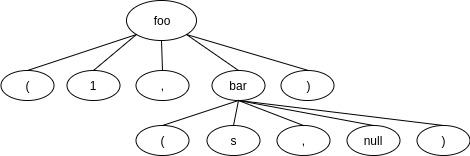
\includegraphics[width=0.5\textwidth]{AST}
	\caption{AST-дерево}
	\label{fig:AST-tree}
\end{figure}

\begin{figure}[h]
	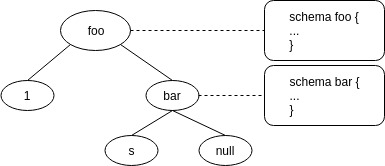
\includegraphics[width=0.5\textwidth]{call-tree}
	\caption{Дерево вызовов}
	\label{fig:call-tree}
\end{figure}

\begin{figure}[h]
	\schema{foo}
	{
		\es {1 == null} $\rightarrow$ \es{Throws IllegalArgumentException} \\
		
		\schema{bar}
		{
			\es{s is String} $\rightarrow$ \es{Returns (s + "1")} \\
			\es{s !is String} $\rightarrow$ \es{Returns (null)}
		}
		{
			\es{== null} $\rightarrow$ \es{Returns (Unit)}
		}
	}
	{}
	
	\caption{Дерево схем}
	\label{fig:schemas-tree}
\end{figure}

\begin{figure}[h]
	\schema{foo}
	{
		\es {1 == null} $\rightarrow$ \es{Throws IllegalArgumentException} \\
		
		\es{s is String && (s + "!") == null}  $\rightarrow$ \es{Returns (Unit)} \\
		
		\es{s !is String && null == null} $\rightarrow$ \es{Returns (Unit)}
	}
	{}
	
	\caption{Плоская схема}
	\label{fig:flat-schema}
\end{figure}

\begin{figure}[h]
	\schema{foo}
	{				
		\es{s !is String} $\rightarrow$ \es{Returns (Unit)}
	}
	{}
	
	\caption{Сокращенная схема}
	\label{fig:reduced-schema}
\end{figure}

\begin{figure}[h]
	\es{s !is String}	
	
	\caption{Результирующая информация}
	\label{fig:info-holder}
\end{figure}

\newpage

\subsection{Применение системы эффектов в компиляторе Kotlin}

\subsubsection{Основы анализа потока данных}

Статический анализ в \lang{Kotlin} тесно связан с фреймворком анализа потока данных (англ. \eng{data-flow analysis}). Это довольно обширная и глубокая тема, и пересказать ее в рамках работы не представляется возможным. Тем не менее, нам необходимо обрисовать эту концепцию хотя бы в общих чертах, поскольку в противном случае разговор об улучшении анализа в \lang{Kotlin} будет слишком неконкретным.

Начнем с понятия графа потока управления (англ. \eng{control-flow graph, CFG}) Каждая инструкция в нем представлена одной вершиной, и если между вершинами $u$ и $v$ есть ребро, то это означает что после инструкции $u$ управление может быть передано 
в инструкцию $v$. 

Рассмотрим простой пример кода:

\begin{minted}{kotlin}
if (x == 0) {
println("True branch")
} else {
println("False branch")
}
println("If-end")    
\end{minted}

Ему соответствует граф потока управления, как на рисунке \ref{control-flow-example}

\begin{figure}
	\centering
	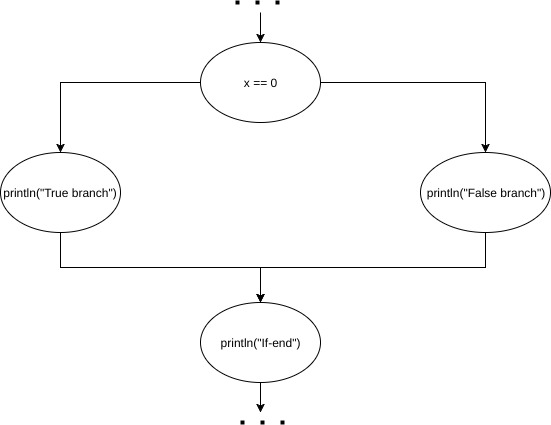
\includegraphics[scale=0.5]{img/control-flow-example}
	\caption{Пример графа потока управления}
	\label{control-flow-example}
\end{figure}


Так, после инструкции, вычисляющей условие в \code{if}, поток управления раздвоился, отражая тот факт, что мы не можем знать при статическом анализе (без дополнительных предположений), какая из веток выполнится. После ветки вновь сливаются в один поток, как и следовало ожидать.

Разумеется, граф потока управления не обязан быть ацикличным -- конструкции \code{for}, \code{while}, \code{goto} (безусловных переход) могут вносить в него обратные ребра.

Важно заметить, что любому возможному пути исполнения в программе обязательно соответствует некоторый путь в CFG, но обратное не верно. Например, путь может проходить через истинную ветку выражения \linebreak \code{if (x == 0) } и через истинную ветку выражения \code{if (x != 0)}, хотя между первым и вторым оператором могло и не быть никаких изменений переменной \code{x}, и иногда это даже можно доказать статически.
Тем не менее, это не нарушает консервативности анализа, поскольку при анализе будет обязательно рассмотрен любой реально возможный путь исполнения. 

Конструкция графов потока управления сама по себе позволяет обнаружить совсем простые ошибки, вроде недостижимого кода из-за неправильного использования безусловных переходов. Однако она становится особо мощной и полезной, если использовать ее вместе с концепцией анализа потока данных.

\begin{definition}
	Анализ потока данных (англ. \eng{data-flow analysis})  -- это метод статического анализа, который основывается на извлечении информации из характеристик и свойств потока данных вдоль различных путей исполнения в программе.
\end{definition}

Основная идея основывается на наблюдении, что в любой момент времени при выполнении программы существует некоторое глобальное состояние, которое состоит из множества всех переменных, их значений, а также другой информации, зависящей от конкретного типа анализа (например, счетчик количества вызовов для функций, статус инициализации переменной, и т.д.). Тогда для каждой точки программы можно ввести понятие \term{значения потока данных} (от англ. \eng{data-flow value}), которое является абстракцией всех возможных глобальных состояний, которые можно наблюдать в данной точке. Для краткости, в дальнейшем мы будем писать DFV вместо <<значение потока данных>>.

В силу того, что потенциально количество возможных путей исполнения в программе может быть бесконечно \cite{dragon-book}, на практике делается два упрощения: во-первых, конкретное DFV не хранит историю, как управление могло придти к этой точке программы, а во-вторых, в зависимости от конкретного анализа, откидывается некоторая излишняя информация. Так, например, при анализе инициализации переменных, нам не важно, какие значения может иметь переменная, и на каких путях исполнения они могли быть получены. Достаточно знать, правда ли, что на любом пути исполнения, достигающем данную точку, данная переменная была инициализирована, или нет. Таким образом, для каждой переменной достаточно просто хранить бинарный флаг, что значительно упрощает реализацию на практике.

Далее, каждой инструкции $s$ соответствует \term{входное состояние} -- глобальное состояние непосредственно перед выполнением инструкции, которое мы будем обозначать $in[s]$, и \term{выходное состояние} -- соответственно, глобальное состояние непосредственно после выполнения инструкции (его мы будем обозначать $out[s]$). Обратим внимание, что выходное состояние для одной инструкции является входным для следующей, с котором она соединена ребром в CFG. Каждому входному (выходному) состояние соответствует некоторое DFV, и в силу предыдущего факта, это отображение является сюръекцией, но не биекцией.

Кроме того, каждая инструкция задает некоторое преобразование, называемое \term{функцией перехода} (англ. \eng{transfer function}), которое по входному состоянию выдает выходное. Конкретный вид преобразования определяется анализом и самой инструкций. 

Таким образом, мы получаем набор уравнений на переменные $in[x]$, $out[x]$ для всех $x \in I$, где $I$ -- множество инструкций в программе. Хотелось бы получить некоторое решение этих уравнений, т.е. множество значений для входных-выходных состояний, удовлетворяющее этим уравнениям. Мы не будем вдаваться в подробности того, как это делается, т.к. это иррелевантно к данной работе, подробней про методы решения систем уравнений на поток данных можно прочитать в канонических источниках: \cite{dragon-book, muchnick}. В дальнейшем нам будет достаточно концепции графа потока управления, входных-выходных состояний и функций перехода.

\subsubsection{Автоматическое приведение типов}

\label{section-upgrading-smartcasts}

Как мы уже говорили, \lang{Kotlin} поддерживает автоматические приведения переменной к более частному типу там, где это возможно. Чаще всего это возможно потому, что если управление дошло до определенной точки в программе, то должны выполняться некоторые ограничения на контекст.

Анализ умных приведений типов полностью основывается на анализе потока данных. Проблемы, описанные в главе 1, связаны с тем, что при извлечении из каждой инструкции начального DFV не учитываются межпроцедурные взаимодействия. Как раз здесь и может помочь система эффектов.

В качестве DFV, для анализа умных приведений типов используется специальный класс \code{DataFlowInfo}, который хранит типовую информацию о переменных из контекста. Кроме того, данный класс поддерживает операции \code{or} и \code{and}, в точности соответствующие операциям, определенным нами в прошлом разделе для приближенных контекстов. Таким образом, этот класс естественно подходит на роль приближенного контекста.

В итоге, в данном пункте с точки зрения системы эффектов не требуется никакой дополнительной работы -- необходимо взять выражение и выполнить серию преобразований, описанных в предыдущем подразделе, используя \code{DataFlowInfo} в качестве приближенных контекстов. Фреймворк анализа потока данных сам обеспечит, чтобы полученная из системы эффектов информация была применена в нужном месте.


\subsubsection{Анализ инициализации переменных}

Анализ инициализации переменных также построен на основе анализа потока данных. Однако здесь для передачи информации из системы эффектов в компилятор нам понадобятся некоторые дополнительные усилия.

Для начала, вспомним, что проблемы с инициализацией появились из-за того, что у компилятора отсутствовала информация о том, что некоторые функции вызывают другие детерминированное число раз. Однако с точки зрения инциализации переменных, нас интересуют не точные количества вызовов каких-то процедур, а более общие понятия, которые мы будем называть \term{статусом вызовов}:

\begin{itemize}
	\item \code{UNKNOWN}, т.е. количество вызовов неизвестно
	
	\item \code{NOT INVOKED}, т.е. ровно ноль вызовов
	
	\item \code{EXACTLY ONCE}, т.е. ровно один вызов
	
	\item \code{AT LEAST ONCE}, т.е. по меньшей мере один вызов
	
	\item \code{AT MOST ONCE}, т.е. не более одного вызова
\end{itemize}

Таким образом, приближенный контекст для анализа инициализации переменных выглядит как отображение из функций в соответствующие им статусы вызовов. Преобразования \code{or} и \code{and} на статусах вызовов определяются довольно безыдейным перебором случаев. Их количество которых может быть несколько оптимизировано при более аккуратном подходе, но это в любом случае остается довольно технической работой, поэтому эти правила вынесены в приложение <TODO: INSERT APPENDIX REF HERE>.

Рассмотрим в качестве примера уже известный нам отрывок кода:

\begin{minted}{kotlin}
	val x: Int
	run {
		x = 42
	}
	println(x)
\end{minted}

Напомним, что изначально такой код не компилировался, поскольку компилятор считал переменную \code{x} в выражении \code{println(x)} не инициализированной. Это происходило из-за того, что для функции \code{run} не было гарантировано, что переданная в нее лямбда \code{ \{ x = 42\} } будет вызвана ровно один раз.

С точки зрения системы эффектов, для вызова функции \code{run} мы можем узнать, что переданная в нее лямбда была вызвана ровно один раз благодаря полученному статусу вызовов \code{EXACTLY ONCE}. Однако передать эту информацию в компилятор не так и просто.

Дело в том, что информация, необходимая для инициализации переменных, выражена в данном случае неявно (сравните это с автоматическим приведением типов, где информация о подтипизации была выражена явно). Если бы мы каким-то образом могли извлекать более явный эффект, например, \code{writes} (означающий, что функция пишет в некоторую переменную), то процесс интеграции был бы ничуть не сложней, чем в случае с приведениями типов.

Теоретически, можно было бы попытаться вывести этот эффект из тела лямбды, а затем аккуратно скомбинировать с эффектом \code{Calls}. Однако с точки зрения дизайна это является некоторым мошенничеством -- инициализация переменной на самом деле происходит в строке \code{x = 42}, в то время как мы приписываем инициализацию в строку вызова \code{run}. Из-за этого могут возникать чисто технические неприятности -- например, если \code{x} и так уже была инициализирована, то ошибка повторной инициализации будет выдана с неправильным номером строки.

Поэтому мы постараемся поступить более <<честно>> -- а именно, донести до компилятора информацию, что поток управления заходит в лямбду и затем выходит из нее, возвращаясь в точку вызова. Иными словами, мы бы хотели добавить ребро из инструкции вызова в начало декларации лямбды, а из конца декларации -- в следующую после вызова инструкцию (см. рисунок \ref{fig:flow-exactly-once-example})

\begin{figure}[h]
	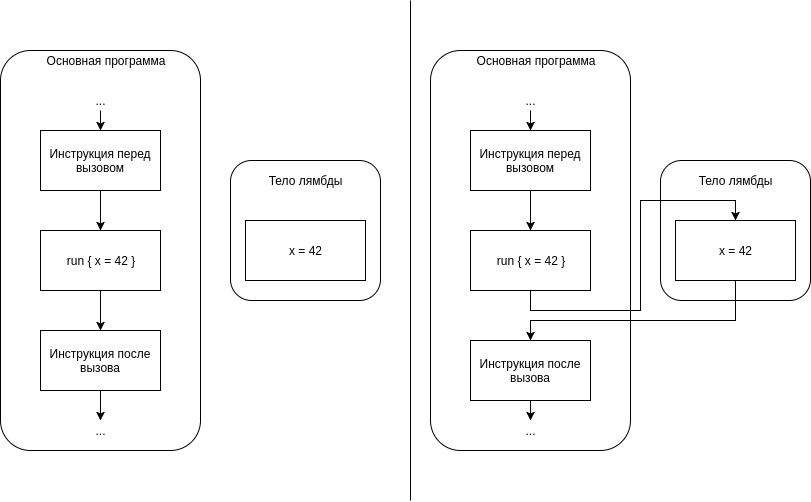
\includegraphics[width=\textwidth]{flow-exactly-once-example}
	
	\caption{Преобразование потока управления. \\ Слева -- исходная ситуация, справа -- после внесения изменений}
	\label{fig:flow-exactly-once-example}
\end{figure}

Этот подход, однако, значительно усложняется, если вместо лямбды используется именованная функция. Рассмотрим, например, следующий пример:

\begin{minted}{kotlin}
	val x: Int
	val block = { x = 42 }
	
	println(x)	// Not initialized yet
	run(block)	
	println(x)	// Initialized once
	run(block)
	println(x)	// Re-initialization
\end{minted}

Именованную функцию можно вызывать несколько раз из различных участков кода -- и каждый вызов может иметь различное значение с точки зрения анализа инициализации. Например, в приведенном выше примере первый вызов корректно инициализирует переменную \code{x}, а вот второй вызов уже вызывает ошибку из-за повторной инициализации. Но поток управления в обоих случаях проходит по одной и той же инструкции, что может опять привести к проблемам с диагностическими сообщениями, и т.д. 

В связи с этим, в рассматриваемой реализации было принято решение ограничиться рассмотрением только анонимных функций. Подчеркнем, что это не является недостатком разработанной системы, а, скорее, некоторыми техническими ограничениями предметной области, не позволяющими в полной мере воспользоваться информацией, поставляемой системой эффектов.

Кроме того, необходимо доставлять в компилятор информации об \code{AT LEAST ONCE}, \code{NOT INVOKED} и \code{AT MOST ONCE}-вызовах. Первый наиболее актуален, т.к. подобные вызовы могут быть использованы для корректной инициализации \code{var}-переменных, допускающих повторное присваивание. К сожалению, подробное описание того, как это было сделано, требует довольно подробного рассмотрения устройства анализа потока данных в компиляторе \lang{Kotlin} и выходит за рамки данной работы. Отметим, однако, что с точки зрения анализа потока данных, \code{AT LEAST ONCE} соответствует циклу \code{do-while} с условием, про которое не известно, сколько раз оно выполнится -- на этом наблюдении и основываются изменения, вносимые в поток управления.


\subsection{Реализация приведений типов в коллекциях}

Напомним, что изначально мы упоминали еще одну проблему, которую мы пока что никак не решили -- это автоматическое приведение типов в коллекциях, например в вызовах типа \code{ list.filter\{ x -> x is String \} }.

Мы не случайно отложили этот вопрос напоследок. Мы уже упоминали, что системы эффектов наиболее хорошо работают со свойствами функций, которые могут быть кратко выражены. Давайте аккуратно сформулируем, каково свойство вызова \code{filter}:

<<Вызов \code{filter} возвращает список, элементами которого являются те элементы исходного списка, на которых переданный предикат вернул \code{true} >>

Это довольно длинная мысль, и она никак не похожа на <<свойство функции, которое может быть выражено кратко>>. Если постараться записать это в более формальном синтаксисе, то можно неожиданно придти к теории множеств:

$$ S.filter(p) = \{ x \in S | p(x) \} $$

Эта запись говорит: \code{S.filter(p)} выдает множество $x$ из $S$ таких, что верен $p(x)$.

Таким образом, для задачи приведения типов в коллекциях лучше всего подходит формализм теории множеств, а не эффектов. Тем не менее, в данной работе мы покажем, как все-таки реализовать поддержку таких понятий в рамках системы эффектов. Помимо чисто научного интереса, это позволит лучше понять границы применимости системы эффектов и того, насколько сложно добавить в описанный фреймворк не свойственные ему понятия.

В дальнейшем мы будем использовать для примера функцию \code{filter}. Для упрощения мы будем рассматривать следующую ее сигнатуру:

\begin{minted}{kotlin}
	fun <T> filter(l: Collection<T>, p: (T) -> Boolean): List<T> {
		...
	}
\end{minted}

\paragraph{Уточнение возвращаемого типа}

Начнем с того, что пока что в нашей системе нет вообще никакого способа сказать, что функция возвращает более конкретный тип, чем описанный в ее сигнатуре. Легче всего это сделать, если расширить семантику \code{Returns}, позволив ему возвращать не только значения, но и типы. Запись \code{Returns(T)} следует понимать следующим образом: функция возвращает \emph{неизвестное} значение типа $T$.

Заметим, что в предложенной в данной работе реализации по некоторым чисто техническим причинам был выбран другой путь, и был введен эффект \code{Hints(variable, type)}, который является полным налогом выражения \code{variable is type}. Их различие состоит в том, что \code{is} может появляться только слева от стрелки импликации, а \code{Hints} -- только справа. В дальнейшем мы будем пользоваться синтаксисом с перегруженным \code{Returns}, для того, чтобы не плодить излишние сущности.

Таким образом, мы уже можем написать часть схемы для \code{filter}, которая выглядит следующим образом:

\schema{filter(l, p)}
{
	\es{true} $\rightarrow$ \es{Returns ( List < ... > )} \\
}{}

Теперь наша задача состоит в том, чтобы вместо многоточия вставить тип, определяемый поведением лямбды, т.е. тип, который имеет аргумент лямбды при условии, что предикат вернул \code{true}. 


\paragraph{Оператор at}

Пусть у нас имеется схема эффектов для предиката \code{p}. Нам необходимо как-то выразить ту мысль, что нас будет интересовать только та часть схемы, которая соответствует случаю, когда предикат вернул \code{true}. Если внимательно посмотреть на эту формулировку, то можно заметить, что она  \emph{в точности повторяет операцию фильтрации схемы}, которую мы определили в пункте \ref{section-back-inference}. 

Таким образом, нам нужно просто предоставить пользователем возможность пользоваться операцией, которая до этого была внутренней для системы эффектов. Для этого мы вводим бинарный оператор \code{at}. Выражение \code{S at E}, где \code{S} -- схема, a \code{E} -- эффект, возвращает схему, соответствующую схеме \code{S} отфильтрованной по эффекту \code{E} как было определено в пункте \ref{section-back-inference}.

Теперь мы можем еще на шаг продвинуться к спецификации \code{filter}:

\schema{filter(l, p)}
{
	\es{true} $\rightarrow$ \es{Returns ( List < p at Returns(true) ... > )}
}{}


\paragraph{Оператор typeOf}

Теперь вместо многоточия осталось вставить конструкцию, которая бы корректно вывела тип, который имеет аргумент лямбды в схеме \code{p at Returns(true)}.

Однако перед тем, как ввести эту операцию, остановимся на одним маленьком нюансе, на котором мы не заострили внимание в прошлом параграфе. Дело в том, что в момент аннотации \code{filter}, невозможно знать, какое имя будет у аргумента лямбды. Следовательно, мы не можем сослаться на этот аргумент.

Если для сравнения посмотреть на спецификацию \code{filter} в терминах теории множеств, то там \emph{вводится} новая переменная $x$ с помощью конструкции $\{ x \in S | P(x) \}$. Мы могли бы поступить по аналогии, и ввести еще одну новую конструкцию для введения переменных -- нечто в духе \code{let x in ...}, навеянное языками семейства ML.

Однако в приведенной реализации удалось этого избежать благодаря тому, что синтаксис \lang{Kotlin} позволяет в сигнатуре функции указать именовать аргументы принимаемых на вход лямбд:

\begin{minted}{kotlin}
	fun <T> filter(s: Collection<T>, p: (arg: T) -> Boolean): List<T> {
		...
	}
\end{minted}

Теперь мы можем ввести оператор \code{typeOf}. Выражение \code{S typeOf V}, где \code{S} -- схема, а \code{V} -- переменная, выдает тип, подтипом которого гарантированно является \code{V} в схеме \code{S}, и из таких наиболее частный. Другими словами, оператор \code{typeOf} в точности соответствует оператору слияния из пункта \ref{section-back-inference}, использующему в качестве приближенных контекстов классы \code{DataFlowValue} из анализа приведений типов в пункте \ref{section-upgrading-smartcasts}. 

Таким образом, полная спецификация \code{filter} выглядит следующим образом:

\schema{filter(l, p)}
{
	\es{true} $\rightarrow$ \es{Returns ( List <(p at Returns(true)) typeOf arg> )}
}{}

В ней, однако, существует одна досадная, чисто техническая ошибка. Дело в том, что при конкретном вызове \code{filter} вместо \code{p} будет подставлена непосредственно некоторая функция, возможно, анонимная. Эта функция может иметь другое мнение на счет того, как должен называться ее первый параметр -- соответственно, и ее схема эффектов будет использовать другое имя для этого параметра. Например, вызов \code{filter(S, \{ x -> x is String \})}, как можно видеть, не упоминает параметра \code{arg} вообще нигде.

В связи с этим, нам необходимо выполнить композицию подстановок -- сначала нужно подставить в схему эффектов \code{filter} все параметры вызова, а затем в тела лямбд нужно подставить корректные аргументы. Для того, чтобы было проще понять, в какие лямбды нужно подставить какое имя, можно более явно специфицировать вызов, и вместо \code{p at ...} писать \code{p(arg) at ...}.

Таким образом, конечный синтаксис записис эффектов для \code{filter} выглядит следующим образом:

\schema{filter(l, p)}
{
	\es{true} $\rightarrow$  \es{Returns ( List <(p(arg) at Returns(true)) typeOf arg> )}
}
{}



\section{Анализ полученной системы}

В данной главе мы постараемся дать некоторую оценку полученной системе, описать ее сильные и слабые стороны, а также очертить границы ее применимости на практике. 

Итак, в данной работе были рассмотрены системы эффектов. Классические эффекты не имеют прикрепленных к ним условий, сообщающих, когда данный эффект будет сгенерирован. Это ведет или к тому, что некоторые функции становится невозможно проаннотировать (например, многие функции возвращают \code{null} только если переданный им аргумент был \code{null}, и такие функции невозможно аннотировать \code{@NotNull}), или же к ограничению свободы анализатора (к примеру, аннотация \code{throws} в \lang{Java} означает, что функция \emph{может} бросить исключение, поэтому отсутствие исключения не дает никакой информации анализатору).

В данной работе была предпринята попытка убрать это ограничение классических эффектов за счет введения т.н. условных эффектов -- т.е. эффектов, к которым прикреплено вызывающее их условие. Это позволяет, с одной стороны, сделать эффекты более строгими -- теперь аннотация \code{Throws} означает, что функция \emph{бросила} исключение, а не \emph{могла} бросить. Более строгие эффекты развязывают руки анализатору, т.к. содержат в себе больше информации -- например, отсутствие исключения позволяет сделать вывод, что соответствующие условие не было выполнено. 

С другой же стороны, введение условий позволяет компенсировать излишнюю строгость самих эффектов -- было бы странно часто видеть функции, для которых просто так верна строгая формулировка аннотации \code{Throws}, в то время как есть вполне жизненная и полезная функция \code{assert}, для которой верна формулировка \code{condition == false -> Throws AssertionError}.

Система условных эффектов естественным образом наследует полезные свойства систем эффектов как таковых: возможность ручной аннотации, в том числе и со стороны пользователя; отсутствие обязательных проверок времени исполнения. Очень важным свойством является то, что вычислительная сложность анализа зависит от количества и типов эффектов, а не от длины кода. Это обеспечивает большую гибкость системы с точки зрения пользователя, позволяя ему самому выбирать между более полным, но медленным анализом, и легковесными аннотациями, не требующими много времени. 

Разработанная система слабо привязана к конкретным эффектам и операторам, что делает ее более гибкой и позволяет легче подстроиться под то или иное конкретное применение. Так, в данной работе в качестве иллюстрации было рассмотрен некоторое малое подмножество операторов языка \lang{Kotlin} и небольшое количество эффектов, необходимых для решения некоторых частных проблем. Пользуясь описанными в работе подходами, можно добавить и другие операторы и эффекты, причем это потребует от минимального до вообще никакого вмешательства в базовые алгоритмы системы (связанные с комбинированием, выводом информации и т.д.). 

В предложенной системе были подробно рассмотрены проблемы вычисления эффектов в присутствии частичных вычислений, что очень актуально для применения подобных систем на практике. Для решения этой проблемы пришлось все же заложить априорное знание о некотором классе эффектов, которые сообщают об успешности или неуспешности вычисления и дают анализатору информацию, необходимую для корректной комбинации эффектов. 

Также не были оставлены без внимания и другие проблемы чисто практического характера. Например, весьма характерной проблемой для условных эффектов является комбинаторный взрыв размера аннотаций при последовательном комбинировании. Для решения этой проблемы в данной работе было намечено два принципиально разных подхода -- первый уменьшает размер схемы без потери информации и основывается на сокращении логических формул. Второй подход был назван аппроксимацией схем и позволяет добиться более сильного уменьшения размера, платя за это потерей информации о некоторых эффектах.

Следует отметить, что как и любой инструмент, система условных эффектов требует соответствующего окружения, способного воспользоваться предоставляемыми ею возможностями. Так, при наблюдении эффектов, система может выводить, при каких условиях на контекст такие эффекты могли быть сгенерированы, получая весьма емкую и ценную информацию об окружении. В данной работе в качестве окружения использовался компилятор языка \lang{Kotlin}, в которым такой информации находилось естественное применение в механизме умных приведений типов.

Кроме того, простота добавления новых синтаксических конструкций не говорит о том, что в систему легко добавить новые понятия в целом. Так, было замечено, что утверждения про коллекции тесно связаны с формализмом теории множеств, и поддержка таких утверждений в системе требует введения ряда дополнительных операторов. Каждый из подобных операторов вводится концептуально просто, но требует некоторой нетривиальной технической работы, тем самым делая добавление одних понятий (не требующих введения новых конструкций) более удобным, чем других. В частности, легче всего добавляются понятия, являющиеся <<побочными эффектами>> в полном смысле этого слова -- например, эффекты вызова другой функции, чтения, записи, и т.д. Чем дальше вводимая абстракция от <<побочного эффекта>>, тем больших усилий она требует для формализации в рамках данной системы.


Таким образом, с точки зрения научной новизны, данное исследование постаралось внести вклад в изучение следующих вопросов:

\begin{itemize}
	\item Условные эффекты с достаточно богатыми условиями
	
	\item Исчисление эффектов в присутствии частичных вычислений
	
	\item Борьба с экспоненциальным ростом размера аннотаций
\end{itemize}


В качестве основных преимуществ полученной системы следует отметить:

\begin{itemize}
	\item Сложность анализа зависит от количества и типов аннотаций, а не от дины кода
	
	\item Расширяемость системы по базовым конструкциям (операторам и эффектам)
	
	\item Гибкость и интенсивность анализа, достигнутая за счет использования условных эффектов
	
	\item Практичность, достигнутая за счет рассмотрения ряда технических вопросов (роста длины аннотаций) и отказа от слишком теоретичных предположений (тотальности вычислений)
\end{itemize}

Недостатками системы являются: 

\begin{itemize}
	\item Недостаточная формализованность, которая может послужить препятствием для понимания, реализации или расширения данной работы
	
	\item Необходимость в использовании дополнительных инструментов и методик для получения практических результатов (например, в данной работе в качестве такого инструмента использовался анализатор компилятора \lang{Kotlin}, выполняющий анализ потока данных)
	
	\item Затруднения при формализации некоторых понятий, не укладывающихся в концепцию эффекта (например, утверждения про свойства коллекции)
\end{itemize}
   
Таким образом, наилучшее применение данная система находит в языках программирования, в качестве побочного инструмента анализа, приходящего на помощь основному в некоторых специальных случаях. В языках программирования наиболее полно раскрываются такие положительные свойства систем эффектов, как возможность ручной аннотации и гибкость в плане затрачиваемых ресурсов, позволяя пользователям языка подстраивать систему под своим нужды.

Разработанная система не должна рассматриваться как средство формальной спецификации (по типу языков спецификаций или даже парадигмы \code{design-by-contract}), несмотря на то, что аннотации эффектов с условиями могут ложно натолкнуть на такую мысль. Для этого данной системе не хватает формальности и выразительности, которые были аккуратно пожертвованы в угоду легковесности и прозрачности.

\section*{Заключение}

В данной работе было рассмотрено расширение классических систем эффектов за счет введение условных эффектов. Были предложены правила комбинации эффектов, предусматривающие возможность масштабирования системы путем добавления новых операторов и эффектов. 

Полученная система наилучшим образом проявила себя при работе с утверждениями, которые хорошо укладываются в классическое понятие <<эффекта>> -- т.е. некоторое изменение в контексте, производимое подпрограммой. Можно сделать вывод, что в систему, при необходимости, можно будет легко добавить большинство классических эффектов: \code{read}, \code{write}, \code{throws}, и др. 

С другой стороны, введение понятий, слабо связанных с побочными эффектами, требует значительно б\a'{o}льших усилий и добавления новых конструкций и операторов. Так, умные приведения типа в коллекциях требуют формализма, являющимся подмножеством теории множеств, и потому укладываются в систему условных эффектов не очень хорошо. Тем не менее, в предложенной системе, технически, имеется возможность выражать и записывать такие понятия.

В качестве примера практической реализации, данная система была реализована в компиляторе языка \lang{Kotlin}. Для учета специфики данного языка (в частности, последовательных вычислений и их частичности), был введен специальный класс эффектов, описывающих исходы вычислений. Знание об этом классе заложено в систему для корректного извлечения эффектов некоторой последовательности вычислений, некоторые из которых завершаются аварийно (с исключением).

За счет добавления этой системы удалось улучшить статический анализ, выполняемый компилятором языка \lang{Kotlin}. В частности, были:

\begin{itemize}
	\item Поддержаны умные приведения типа, извлекающие информацию из выражений в условных конструкциях и включающих в себя вызовы функций.
	
	\item Поддержаны умные приведения типа, опирающиеся на факт (не)успешного завершения функции (например, в вызовах \code{assert}). 
	
	\item Поддержаны умные приведения типа в коллекциях (например, в вызовах вида \code{Collection<T>.filter})
	
	\item Улучшены существующие в компиляторе диагностики (например, об инициализации переменных) за счет эффектов, описывающих, что функция в ходе своего выполнения вызовет некоторую другую детерминированное число раз. 
\end{itemize}

Также был реализован вывод эффектов из простых выражений.

В качестве возможных направлений развития следует отметить:

\begin{itemize}
	\item Расширение системы за счет добавления других конструкций логики: кванторы, импликации (в явном виде), предикаты
	
	\item Исследование других эффектов: например, связанных с многопоточностью, вводом-выводом, чтением-записью в переменные, и т.д.
	
	\item Улучшение системы автоматического вывода эффектов.
\end{itemize}

% Use relative to `./out` paths because of shitty LaTeX (BibTeX) build-system
\bibliographystyle{./../BibTeX-Styles/ugost2008ls}
\bibliography{./../bib/diploma}

\begin{appendices}

\section{Грамматика}

\label{appendix-es-grammar}

\begin{minted}{text}
grammar EffectSystem;


// Entry-point
effectSchema
    : EOF
    | clause (SEMI clause)*
    ;

clause
    : expression '->' effectsList
    ;


// Expressions

expression
    : conjunction (disjunctionOperator conjunction)*
    ;

conjunction
    : equalityComparison (conjunctionOperator equalityComparison)*
    ;

equalityComparison
    : comparison (equalityOperator comparison)*
    ;

comparison
    : namedInfix (comparisonOperator namedInfix)*
    ;

namedInfix
    : additiveExpression (inOperation additiveExpression)*
    | additiveExpression atOperation effect
    | additiveExpression (isOperation type)?
    ;

additiveExpression
    : multiplicativeExpression (additiveOperator multiplicativeExpression)*
    ;

multiplicativeExpression
    : prefixUnaryExpression (multiplicativeOperator prefixUnaryExpression)*
    ;

prefixUnaryExpression
    : prefixUnaryOperation* postfixUnaryExpression
    ;

postfixUnaryExpression
    : atomicExpression postfixUnaryOperation*
    ;

atomicExpression
    : '(' expression ')'
    | literalConstant
    | SimpleName
    ;

disjunctionOperator
    : '||'
    ;

conjunctionOperator
    : '&&'
    ;

equalityOperator
    : EQEQ
    | EXCLEQ
    ;

comparisonOperator
    : LT | GT | LEQ | GEQ
    ;

additiveOperator
    : PLUS | MINUS
    ;

multiplicativeOperator
    : MUL | DIV | PERC
    ;

prefixUnaryOperation
    : MINUS | PLUS
    | MINUSMINUS | PLUSPLUS
    | NOT
    ;

postfixUnaryOperation
    : PLUSPLUS | MINUSMINUS | EXCLEXCL
    | callSuffix
    ;

callSuffix
    : '(' (expression (',' expression)*)? ')'
    ;

inOperation
    : 'in' | '!in'
    ;

isOperation
    : 'is' | '!is'
    ;

atOperation
    : 'at'
    ;


// Effects

effectsList
    : effect (',' effect)*
    ;

effect
    : throwsEffect
    | returnsEffect
    | callsEffect
    | hintsEffect
    ;

throwsEffect
    : 'Throws' type
    ;

returnsEffect
    : 'Returns' '(' (expression | UnknownLiteral ) ')'
    ;

callsEffect
    : 'Calls' '(' callsRecord (';' callsRecord)* ')'
    ;

callsRecord
    : SimpleName IntegerLiteral;

hintsEffect
    : 'Hints' '(' SimpleName ',' typeExpression ')'
    ;

literalConstant
    : BooleanLiteral
    | IntegerLiteral
    | StringLiteral
    | NullLiteral
    | UnitLiteral
    ;

typeExpression
    : type
    | typeOfOperator
    ;

type
    : SimpleName typeParametersList?
    ;

typeOfOperator
    : expression 'typeOf' SimpleName
    ;

typeParametersList
    : '<' typeExpression (',' typeExpression)* '>'
    ;

BooleanLiteral
    : 'true'
    | 'false'
    ;

NullLiteral : 'null';

UnknownLiteral : 'unknown';

UnitLiteral : 'unit';


// String literals
StringLiteral
    :   '"' StringCharacters? '"'
    ;

fragment
StringCharacters
    :   StringCharacter+
    ;

fragment
StringCharacter
    :   ~["\\]
    |   EscapeSequence
    ;

fragment
EscapeSequence
    :   '\\' [btnfr"'\\]
    |   OctalEscape
    |   UnicodeEscape
    ;

fragment
OctalEscape
    :   '\\' OctalDigit
    |   '\\' OctalDigit OctalDigit
    |   '\\' ZeroToThree OctalDigit OctalDigit
    ;

fragment
UnicodeEscape
    :   '\\' 'u' HexDigit HexDigit HexDigit HexDigit
    ;

fragment
ZeroToThree
    :   [0-3]
    ;

// Numeric literals

//TODO add hex/binary/octal integers
IntegerLiteral
    :   DecimalIntegerLiteral
    ;

fragment
DecimalIntegerLiteral
    :   DecimalNumeral IntegerTypeSuffix?
    ;

fragment
IntegerTypeSuffix
    :   [lL]
    ;

fragment
DecimalNumeral
    :   '0'
    |   NonZeroDigit (Digits? | Underscores Digits)
    ;

fragment
Digits
    :   Digit (DigitOrUnderscore* Digit)?
    ;

fragment
Digit
    :   '0'
    |   NonZeroDigit
    ;

fragment
NonZeroDigit
    :   [1-9]
    ;

fragment
DigitOrUnderscore
    :   Digit
    |   '_'
    ;

fragment
Underscores
    :   '_'+
    ;

fragment
OctalDigit
    :   [0-7]
    ;

fragment
HexDigit
    :   [0-9a-fA-F]
    ;

// Identifiers

SimpleName
    :   JavaLetter JavaLetterOrDigit*
    ;

fragment
JavaLetter
    :   [a-zA-Z$_] // these are the "java letters" below 0x7F
    |   // covers all characters above 0x7F which are not a surrogate
        ~[\u0000-\u007F\uD800-\uDBFF]
    |   // covers UTF-16 surrogate pairs encodings for U+10000 to U+10FFFF
        [\uD800-\uDBFF] [\uDC00-\uDFFF]
    ;

fragment
JavaLetterOrDigit
    :   [a-zA-Z0-9$_] // these are the "java letters or digits" below 0x7F
    |   // covers all characters above 0x7F which are not a surrogate
        ~[\u0000-\u007F\uD800-\uDBFF]
    |   // covers UTF-16 surrogate pairs encodings for U+10000 to U+10FFFF
        [\uD800-\uDBFF] [\uDC00-\uDFFF]
    ;


WS  :  [ \t\r\n\u000C]+ -> skip
    ;

EOL : '\r'? '\n';

SEMI : ';';

LT : '<';
GT : '>';
LEQ : '<=';
GEQ : '>=';
PLUS : '+';
MINUS : '-';
MUL : '*';
DIV : '/';
PERC : '%';
PLUSPLUS : '++';
MINUSMINUS : '--';
NOT : '!';
EXCLEXCL : '!!';
EQEQ : '==';
EXCLEQ : '!=';
\end{minted}



\end{appendices}

\end{document}
